\documentclass[aps,prd,amsmath,floats,floatfix, twocolumn,
superscriptaddress,nofootinbib,showpacs]{revtex4-1}

\usepackage[colorlinks, pdfborder={0 0 0}, plainpages=false]{hyperref}
\usepackage{graphicx}
\usepackage{xspace}
\usepackage[usenames,dvipsnames]{color}
\usepackage{amssymb}
\usepackage[dvipsnames]{xcolor}
\usepackage{placeins}
% \usepackage[switch,columnwise]{lineno} 
\usepackage{lineno}
\newcommand{\roughly}{\mathchar"5218\relax} % Different from \sim in spacing

% Macros for text changes
\newcommand{\red}{\textcolor{red}}
\newcommand{\dan}[1]{\textcolor{WildStrawberry}{#1}}
\newcommand{\Mark}[1]{\textcolor{Cerulean}{#1}}
\newcommand{\larry}[1]{\textcolor{OliveGreen}{#1}}
\newcommand{\bela}[1]{\textcolor{Blue}{#1}}
\newcommand{\saul}[1]{\textcolor{Orange}{#1}}
\newcommand{\prayush}{\textcolor{red!40!black}}

% Macros for text notes and comments
\newcommand{\Note}[1]{\textcolor{blue}{\textbf{[#1]}}}
\newcommand{\D}{\mathrm{d}}
\newcommand{\lambdans}{\Lambda_\mathrm{NS}}
\newcommand{\dlambda}{\delta\Lambda}

\newcommand{\ii}{\mathrm{i}}
\newcommand{\chibh}{\chi_\mathrm{BH}}
\newcommand{\chins}{\chi_\mathrm{NS}}
\newcommand{\mbh}{m_\mathrm{BH}}
\newcommand{\mns}{m_\mathrm{NS}}
\newcommand{\mchirp}{\mathcal{M}_c}
\newcommand{\LL}{\mathcal{L}}
\newcommand{\deff}{D_\mathrm{eff}}
\newcommand{\arr}{\mathtt{r}}


\newcommand{\Caltech}{\affiliation{Theoretical Astrophysics 350-17,
    California Institute of Technology, Pasadena, CA 91125, USA}}
\newcommand{\Cornell}{\affiliation{Center for Radiophysics and Space
    Research, Cornell University, Ithaca, New York 14853, USA}}
\newcommand{\CITA}{\affiliation{Canadian Institute for Theoretical
    Astrophysics, 60 St.~George Street, University of Toronto,
    Toronto, ON M5S 3H8, Canada}} %
\newcommand{\GWPAC}{\affiliation{Gravitational Wave Physics and
    Astronomy Center, California State University Fullerton,
    Fullerton, California 92834, USA}} %
\newcommand{\AEI}{\affiliation{Albert Einstein Institute,
Am M\"uhlenberg, G\"olm, Germany}} %
\newcommand{\CIFAR}{\affiliation{Canadian Institute for Advanced Research, 
    180 Dundas St.~West, Toronto, ON M5G 1Z8, Canada}} %



    
\newcommand{\NS}{\mathrm{NS}}
%%%%%%%%%%%%%%%%%%%%%%%%%%%%%%%%%%%%%%%%%%%%%%%%%%%%%%%%%%%%%%%

\begin{document}
\linenumbers

\title{
Measuring neutron star tidal deformability with Advanced LIGO: a Bayesian analysis of mixed binary observations
}

\author{Prayush Kumar}\CITA\email{prkumar@cita.utoronto.ca}
\author{Michael P\"urrer}\AEI
\author{Harald P. Pfeiffer}\CITA\CIFAR\AEI

\date{\today}

\begin{abstract}
The pioneering discovery of gravitational waves (GW) by Advanced LIGO has ushered
us into an era of observational GW astrophysics. Compact binaries remain the 
primary target sources for GW observation, of which neutron star - black hole 
(NSBH) binaries form an important subset.
% 
GWs from NSBH sources carry signatures of (a) the star's tidal distortion by
the companion black hole (BH) during inspiral, and (b) its tidal disruption
(if that happens) near merger.
%
In this paper, we present a Bayesian study of the measurability of
neutron star (NS) tidal deformability $\lambdans\propto (R/M)_\mathrm{NS}^{5}$
from GW observation(s) of disruptive NSBH coalescences, taking into account the
crucial effect of BH spins.
% 
First, we find that if BHBH templates are used to estimate source 
parameters for an NSBH signal, a significant bias is introduced in the 
inference if the signal-to-noise ratio (SNR) is greater than $\simeq30$.
% 
Second, we find that if we are to get a loud signal with SNR $\gtrsim 23$, 
we can put a factor of two bound on $\lambdans$.
% 
Finally, we study the improvement in our measurement of $\lambdans$ from 
multiple observations. Using an approximately astrophysical population, 
we find that (i) the median measured $\lambdans$ catches up to within
$10\%$ of the true value in approximately $20$ observations; (ii) in the same
number of observations, the associated $90\%$ confidence intervals shrink to
$\pm 50\%$ of the true value.
% 
We find these results encouraging, and recommend that an effort to 
measure $\lambdans$ be taken within the LIGO-Virgo Collaboration once
we begin to detect NSBH coalescences.
\end{abstract}

\pacs{}
% 04.25.D- Numerical relativity
% 04.25.dg Numerical studies of black holes and black-hole binaries
% 04.25.Nx Post-Newtonian approximation; perturbation theory; related approximations 
% 04.30.-w Gravitational waves (see also 04.80.Nn Gravitational wave detectors and experiments)
% 04.30.Db Wave generation and sources 
% 02.70.Hm Spectral methods

\maketitle

%%%%%%%%%%%%%%%%%%%%%%%%%%%%%%%%%%%%%%%%%%%%%%%%%%%%%%%%%%%%%%%%%%%%%%%%%%%%%%%
\section{Introduction}\label{s1:introduction}
%%%%%%%%%%%%%%%%%%%%%%%%%%%%%%%%%%%%%%%%%%%%%%%%%%%%%%%%%%%%%%%%%%%%%%%%%%%%%%%

The Advanced LIGO (aLIGO) observatories completed their first observing run ``O1''
early-2016, operating at a factor of $3-4$ higher gravitational-wave
(GW) strain sensitivity than their first-generation 
counterparts~\cite{Shoemaker2009}.
% 
During O1, they made the first terrestrial observation of gravitational 
waves~\cite{LIGOVirgo2016a}. Emitted by a pair of coalescing black holes, these
waves heralded an era of observational GW astrophysics as they traveled 
through Earth.
% 
Towards the end of this decade, we expect aLIGO to reach its design sensitivity.
In addition to the US-based efforts, we also expect the French-Italian detector Advanced
Virgo~\cite{aVIRGO,aVirgo2}, Japanese detctor KAGRA~\cite{kagra,Somiya:2011np},
and LIGO-India~\cite{2013IJMPD..2241010U} to begin observing at comparable
sensitivities within a few years. With a global network of sensitive GW
 observatories, we can expect GW astronomy to face significant developments over the
coming years.
% 
% At design sensitivity, we expect aLIGO to observe $\sim 70$ compact binary
% mergers a year~\cite{Abadie:2010cf}.

% \red{
% Text about CBCs. How was each type observed so far?
% }
Coalescing compact binaries (both monolithic and mixed) of stellar-mass black
holes (BH) and neutron stars (NS) are the primary targets for the second
generation GW detectors~\cite{Timmes:1995kp,Fryer:1999mi,RevModPhys.74.1015,
2010ApJ...714.1217B,2010ApJ...715L.138B,Dominik:2014yma,Belczynski:2006zi,
2012ApJ...749...91F,
Wex:1998wt,1991ApJ...379L..17N,Mandel:2015spa,Abbott:2016nhf}.
A monolithic binary of black holes was recently observed by 
aLIGO~\cite{LIGOVirgo2016a}. Previously, stellar-mass black holes had only 
been observed by inference in mixed binaries with stellar companion (through
electromagnetic observations of the companion)~\cite{Lewin2010,
Remillard:2006fc,Fragos:2010tm}.
Neutron stars, on the other hand, have had numerous sightings. Thousands of
electromagnetically emitting neutron stars, or pulsars, have been 
documented~\cite{Manchester:2004bp},
in varied situations: as radio pulsars~\cite{Lattimer:2012nd,Manchester:2004bp},
in binary systems with stellar companions~\cite{1971ApJ...169L..23M,
Bond:2002eh,Lattimer:2012nd,Manchester:2004bp},
and in monolithic neutron star binaries~\cite{Hulse:1975uf,Taylor:1982wi,
Weisberg:2010zz,Lattimer:2012nd,Manchester:2004bp}.
Mixed binaries of black holes and neutron stars, is an astrophysically
interesting class of systems~\cite{Wex:1998wt,
1991ApJ...379L..17N,Janka1999,Fryer:2015jpa}, that is yet undetected.
We expect to observe $\mathcal{O}(10)$ mixed binaries per year with
aLIGO~\cite{Abadie:2010cf}.


% \prayush{
% The actual masses of
% astrophysical black holes are uncertain, but observations and
% population synthesis studies suggest that BHs formed from stellar
% core-collapse can have masses up to and higher than
% $34M_\odot$~\cite{2008ApJ...678L..17S,2010ApJ...714.1217B}.  Also,
% recent measurements using continuum fitting and X-ray reflection
% fitting suggest that black holes can have high spin, with the BH
% angular momentum in dimensionless units exceeding
% $0.8$~\cite{2011ApJ...742...85G,2012MNRAS.424..217F,Gou:2013dna,
%   2009ApJ...697..900M,McClintock:2006xd,Miller:2009cw,McClintock:2013vwa}.
% }
% % 

% \red{
% Text describing BHNS disruption and accretion dynamics.
% }

% Most of the matter falls into the BH in ~1ms. But the disk itself has an
% accretion timescale of ~100ms-1s. The disk-BH system is the expected engine
% for a SGRB, through the production of a relativistic jet. The unbound material,
% on the other hand, is responsible for an EM signal in the infrared/optical, 
% powered by radioactive decays in the ejecta. And possibly a radio afterglow
% through interactions with the ISM. But not gamma-rays (unless you are referring
% to the very small amount of material ejected in the jet, but that's not what
% people usually mean when talking about material unbound by the merger).
% 


NSBH binaries are of interest for multiple reasons. For instance,
they have been long associated with (as possible progenitors of) short
Gamma-ray Bursts (SGRBs)~\cite{eichler:89,1992ApJ...395L..83N,moch:93,Barthelmy:2005bx,
2005Natur.437..845F,2005Natur.437..851G,Shibata:2005mz,Paschalidis2014,
Tanvir:2013}. Depending on their equation of state (EoS), NSs can get disrupted by
the tidal field of their companion BHs. Once disrupted, most of the NS
material falls into the hole over an $\mathcal{O}(1$ms$)$ time-scale,
with the rest partly getting ejected as unbound material
% (kilonovae, r-process material),
and partly forming an accretion disk around the BH.
% 
This short lived ($0.1-1s$) disk-BH system is hypothesized to drive SGRBs
through the production of relativistic jets~\cite{Foucart:2015a,
Lovelace:2013vma,Deaton2013,Foucart2012,Shibata:2005mz,Paschalidis2014}.
% 
However, whether or not such a system forms depends also on the nature of
the BH. For e.g., massive BHs (with $\mbh\gtrsim 10M_\odot$), as well as BHs with
large retrograde spins, tend to swallow the NS whole without forming a
disk~\cite{Foucart:2013psa}. 
% 
On the other hand, {\it low-mass} BHs with $\mbh\in[3M_\odot, 7M_\odot]$, 
can disrupt their companion NSs much before merger, forming long-sustained disks
that are required to sustain 
SGRBs~\cite{Shibata:2007zm,2010PhRvD..81f4026F,Lovelace:2013vma,Kawaguchi:2015}.
% 
% Such systems additionally leave a strong imprint on the emitted GW signal.
A {\it coincident} detection of both GWs and gamma-rays from an NSBH merger,
whenever it happens, will
provide us with a uniquely opportunity to confirm this hypothesized link between
NSBH mergers and GRBs~\cite{Abbott:2016wya}.


% \red{
% Text focusing on tides
% }

Another question that NSBH mergers can help answer is `what is the 
nature of matter at nuclear densities', i.e. `what is the EoS of NS material'?
This is what we will focus on in this paper.
% 
During the course of early inspiral, the tidal field of the BH produces a
deformation in its companion NS. The quadrupolar moment of the star associated
with this deformation also depends on its material properties, through an EoS-dependent
tidal deformability parameter $\lambdans$. This induced quadrupolar moment
changes over the orbital time-scale, resulting in the emission of GWs in {\it
coherence} with the orbital waves.
These waves draw more energy from the orbit and increase the inspiral rate (as
compared to an equivalent BBH)~\cite{Flanagan2008}.
% The coherence of GW emission between stellar and orbital waves drains energy 
% more rapidly from the orbit and increases the inspiral rate (compared to a
% BBH)~\cite{Flanagan2008}.
% 
% We know the leading and next-to-leading order terms in post-Newtonian (PN)
% theory that capture this effect~\cite{Vines2011}, entering binary phasing at
% $5$PN order.
% 
Closer to merger, the strong tidal field of the BH can disrupt the NS. The
quadrupolar moment of the disrupted binary system falls monotonically over a
millisecond time-scale~\cite{Kyutoku:2010zd,Lackey:2013axa,Lovelace:2013vma,Foucart:2015a,
Pannarale:2015jia}.
% 
This penultimate stage also depends strongly on the internal structure and energy
transport mechanism of the NS~\cite{}.

% This penultimate stage carries the strongest signature in the GW spectrum, and
% can possibly be accompanied by SGRBs. 
% The final stage is a BH, whose quasi-normal
% modes may (or not) be strongly excited~\cite{FoucartEtAl:2011,Lackey:2013axa}.



% During early inspiral, the (weak) tidal field of the BH deforms its companion
% NS.
% % , thereby exciting its resonant oscillation modes.
% The resulting induced quadrupolar moment of the star is proportional to the
% tidal field of its companion,
% % through the relation $Q_{ij} = -\lambda\mathcal{E}_{ij}$,
% with $\lambdans$ the EoS-dependent proportionality constant. $\lambdans$ is the
% NS's tidal deformability parameter, related to its dimensionless Love number
% $k_2$ and radius $R_\mathrm{NS}$ as $\lambdans:=\frac{2}{3G}k_2 R_\mathrm{NS}^5$.
% % 
% Over the course of inspiral, the change in NS's quadrupole moment results in 
% the emission of GWs that are coherent with the orbital waves.
% % 
% 



% \red{
% Insert paragraph describing impact on GWs
% }
% 
% \red{
% Make clear the distinction between Fischer matrix studies and Bayesian ones. 
% Explain the differences. this is important as it sets the stage for for what is
% new in this paper.
% } 
% - Describe how waves are affected in each stage for a NSBH. 
% - Describe what past work has studied and how?
% - Do we need to compare with BNS.. Maybe in passing, say `` In comparison, for BNS we expect to measure EoSs within 20 detections.

Gravitational waves emitted by coalescing NSBH binaries carry subtle hints of
the NS EoS from inspiral through to merger. During early inspiral, the tidal
dephasing is relatively weak and appears as a $5^{th}$ Post-Newtonian (PN)
order effect~\cite{Vines2011}. Closer to merger, a disruptive fate of the NS
can result in a strong suppression of GW emission above a cut-off 
frequency~\cite{Pannarale:2015jia}. Some past studies of tidal measurements
with NSBH binaries have used PN inspiral-only waveforms~\cite{Maselli:2013rza}.
In doing so, however, (i) they ignore the merger signal which could contain significant
information for NSBHs, and (ii) the errors due to unknown vaccum terms in PN 
waveforms could dominate over the tidal terms themselves~\cite{Barkett2015,
Yagi:2014}.
% 
Some other studies that account for merger effects via the use of complete
numerical simulations~\cite{Foucart:2013psa}, are limited in the binary
parameter space they sample.
% 
Others, that do the same through the use of phenomenological waveform
models~\cite{Lackey2011,Lackey:2013axa} use the Fisher matrix to estimate
$\lambdans$ measurement errors. Fisher matrix estimates are known to be
unreliable at realistic signal-to-noise ratios (SNR)~\cite{Vallisneri:2007ev},
such as those as we might expect in the upcoming observing runs of GW
detectors~\cite{Abadie:2010cf}.




% A large fraction of past work aimed at measuring NS matter effects from GW
% signals has consisted of inquiries about binary neutron stars (BNS)~\cite{
% Lee1999a,Lee1999b,Lee2000,oechslin:07,Read:2008iy,Markakis:2010mp,Markakis:2011vd,
% stergioulas:11,East:2011xa,Lackey2014,Wade:2014vqa,Bauswein:2014qla}.
% % 
% % It has shown~\cite{DelPozzo:13,Chatziioannou:2015uea,Agathos:2015a} that
% % with $20-30$ BNS observations, aLIGO would begin to distinguish between hard,
% % moderate and soft candidate equations of state.
% % 
% % These studies rely on the PN 
% % description of BNS dynamics, which is reasonable since BNSs merge at very high
% % frequencies and most of their signal power resides in inspiral.
% % 
% During early inspiral the tidally induced waves are weak in strength,
% as appropriate for an effect that enters binary phasing at $5^{th}$
% Post-Newtonian (PN) order~\cite{Vines2011}. During late-inspiral and merger,
% a disruptive fate of the NS could result in significant suppression of the
% emitted GWs~\cite{}.
% % 
% % The difficulty in discerning NS matter effects in an NSBH coalescence from its
% % GW signal lies in distinguishing it reliably from a BBH signal, since the 
% % difference between the two is either subtle (during inspiral) or short-lived
% % (disruption and merger).
% % 
% The earlier in inspiral the NS disrupts, the more orbits there are over which
% its effects are manifest in the GW signal.
% % 
% In addition, NSBHs merge at relatively lower frequencies than BNS, and their
% disruption during late-inspiral occurs at frequencies where aLIGO has
% relatively more resolving power. This, combined with a shorter inspiral,
% means that the merger portion of NSBH signals is relatively more valuable for
% measuring $\lambdans$. 


In this paper we study the measurability of neutron star's tidal deformability
from realistic binaries of {\it low}-mass BHs and NSs by aLIGO. We also probe
how tidal effects affect the estimation of other binary parameters for the same
class of systems. This study improves upon previous work in the following ways.
% 
First, we include tidal effects during inspiral and merger in a consistent
way, by using the waveform model of Lackey et al.~\cite{Lackey:2013axa}
(abbreviated henceforth to ``LEA+'').
% 
Second, we include the effect of black hole spin on tidal GW signals, in
addition to the effect of BH mass, NS's deformability, and the SNR.
% 
Third, we perform a complete Bayesian analysis, instead of using the Fisher matrix
approximation.
% 
Fourth, we explore how our measurement errors decrease as we gain information
from multiple (realistic) events.


We first probe the effect of ignoring tidal effects in parameter 
estimation on the recovery of non-tidal binary parameters, such as 
component masses and spins. This is the case of current and planned aLIGO
efforts.
To do so, we first use the LEA+ model to generate a set of realistic signals;
and then use non-tidal (BBH) waveform filters to estimate the underlying
binary masses and spins with a Markov-chain Monte Carlo.
% 
% \red{
% MOVE the following to SUMMARY. Here, keep 1-2 sentences:
We find that, for individual events, ignoring tidal effects will affect
mass-estimation only marginally; only for very loud signals (SNRs $\gtrsim 30$)
will the systematic biases be large enough to exceed the underlying
statistical uncertainty. Furthermore, detection searches can ignore tidal
effects without loss of sensitivity.
% }


% \red{
% Somewhat reduce discussion of results. Discuss in order of probability, starting
% with low SNR, ending with exceptional events.
% }

% \prayush{
Second, we study the ability of aLIGO to constrain neutron star tidal 
deformability with a single observation of NSBH merger. For this, we
use the same setup for signal waveforms as before, but replace the filter
template model with one that includes tidal effects from inspiral
through to merger (i.e. LEA+)~\cite{Lackey:2013axa}. For most binaries with
BH masses outside of the mass-gap and/or realistic signal-to-noise
ratios (SNR), we find it difficult to put better than a factor of $2$ bound
on $\lambdans$ with a single observation. As we can see from
Fig.~\ref{fig:TT_LambdaCIWidths90_0_Lambda_SNR}, it is only at SNRs 
$\rho\gtrsim 20-30$ (under otherwise favorable circumstances) that we are able
to bring this down to a $\pm 75\%$ bound on $\lambdans$. For signals louder
than $\rho =30$, we can constrain $\lambdans$ to a much more meaningful degree
(within $\pm 50\%$ of its true value).
% For more realistic SNRs and BH parameters, a single measurement is 
% for $\lambdans$ is accompanied with a $\sim\pm150+\%$. uncertainty.
% }
While this is discouraging at first, we turn to ask: what if we combine
information from a population of low-SNR observations?



% \red{
% BEgin this paragraph by pointing out that EOS is universal among all NSs. 
% Therefore, one universal $\lambdans$ vs $\mns$ curve. Therefore, by combining
% multiple BHNS events, expect to measure $\lambdans$ better than with any 
% single BHNS event.
% }
% % \prayush{
The EoS of matter at nuclear densities is believed to be universal among all
neutron stars. The Tolman-Oppenheimer-Volkoff equation would then predict that NS
properties satisfy a universal relationship between $\lambdans$ and $\mns$. As
the final part of
this paper, we combine information from multiple observations of realistic NSBH
systems and perform a fully-Bayesian analysis of how our estimation of
$\lambdans$ changes as we accumulate detections. This is similar to an earlier
study~\cite{DelPozzo:13} aimed at binary neutron stars.
% % }
% % 
% \red{
% MOVE into later sections. Keep here only 1-2 informational sentences.
% }
% % 
We restrict ourselves to a population of NSs with masses clustered very tightly
around $1.35M_\odot$ (with a negligible variance), and negligible spins. We
sample different nuclear EoSs by sampling entire populations fixing different
values for the NS tidal deformability.
% These values correspond to a hard EoS at the lower end, and a soft EoS at the upper.
For all populations, we take source locations to be uniformly distributed in
spatial volume, and source orientations to be uniform on a $2-$sphere. To
summarize, we find the following:
% 
(a) Our best estimate for $\lambdans$ improves much faster than our statistical
uncertainties. Within $10-20$ detections, the median measured value of
$\lambdans$ lies within $10\%$ of the actual value.
(b) Measurement uncertainties for $\lambdans$, on the other hand, depend on
$\lambdans$ itself. We find that for hard equations of state (with 
$\lambdans\geq 1000$), $10-20$ observations are sufficient to constrain
$\lambdans$ within $\pm 50\%$. For softer equations of state, the same level
of certainty would require substantially more ($25-40$) observations.
% 
(c) Further, if the astrophysical ``mass-gap'' is real, we find that $20-50\%$
additional observations would be required to attain the same measurement
accuracy as above. And, (d) putting tighter constraints on the $\lambdans$ of a
population would require $50+$ NSBH observations, in any scenario.
% 
All of the above is possible within a few years of design
aLIGO operation~\cite{Abadie:2010cfa}.

% \red{
% MOVE to SUMMARY, only keeping 2-4 sentences here. Also, paradigm A/B barely
% matters. Therefore, first describe the common results, then point out how the
% presence/absence of mass gap modifies them.
% }
% 
% % \prayush{
% In addition, we probe two paradigms, one
% that allows for BH masses to lie within the astrophysical mass-gap (paradigm
% A), and one that does not (paradigm B).
% % 
% For paradigm A, we find the following: (i) for the softer equations of state
% that result in less deformable neutron stars, $15-20$ detections are sufficient
% for our median measured value of $\lambdans$ to lie within $10\%$ of the true
% value. (ii) For NSBH populations with more deformable NSs
% ($\lambdans\geq 1000$), the same is achievable within as few as $10$ realistic
% observations. (iii) The statistical uncertainty associated with $\lambdans$
% measurement can be restricted to be within $\pm50\%$ using $10-20$ observations
% when $\lambdans\geq 1000$), and using $25-40$ observations for softer equations
% of state. All of the above is possible within a few years of design
% aLIGO operation~\cite{Abadie:2010cfa}, if astrophysical BHs do indeed have
% masses between $\leq 5M_\odot$ (i.e. in the mass-gap). However, further
% restricting $\lambdans$ will require $50+$ NSBH observations.
% % 
% For paradigm B, we find the information accumulation to be somewhat slower.
% While the quantitative inferences for $\lambdans\geq1000$ populations are
% not affected significantly, we find $\mathcal{O}(10-20)\%$ more events are
% required to attain the same measurement accuracy as under paradigm A.
% % 
% We conclude that within as few as $20-30$ observations of disruptive NSBH
% mergers, aLIGO will begin to place interesting bounds on NS deformability.
% This, amongst other things, will allow us to rank different equations of 
% state for neutron star matter from most to least likely, with a few years'
% time-scale.
% % }




% \red{
% The following numerical details disrupt the flow of the text. MOVE after
% description of analyses.
% }

% \prayush{
In this paper, we restrict our parameter space to span mass-ratios
$q:=\mbh/\mns\in[2,5]$, BH spin (aligned with orbit)
$\chibh\in[-0.5, +0.75]$, and dimensionless NS tidal deformability 
$\lambdans:= G\left(\frac{c^2}{G \mns}\right)^5\lambda \in[500, 2000]$.
The mass of NS for signals (and not templates) is fixed to $1.35M_\odot$ 
throughout~\cite{stellarcollapsemass}. Similarly, their spin is taken to be
negligible~\cite{Miller:2014aaa}. Signal strength is sampled over a range of
SNR $\rho\in[10, 70]$.
% }
% 
Further, we note that our results are applicable for the design sensitivity
LIGO instruments ($2018-19$).
We also note that the parameter space probed is somewhat restricted by the
domain of applicability of the LEA+ model which we use as filters.
Finally, the accuracy of our quantitative results depends on the reliability of
the same waveform model, which is the only one available of its kind in 
current literature. A more recent work~\cite{Pannarale:2015jka}, improves on
the GW amplitude model, which however needs to be augmented with a compatible
phase model. 
% In addition, accuracy of the underlying numerical simulations 
% used to calibrate the waveform model used here have not been verified against 
% independent codes so far.
% It is therefore difficult to assess the combined modeling error and its effect
% on our results. they are, therefore, limited by the limitations of our
% waveform model. 
However, we expect the combined effect of modeling errors to not change our 
broad qualitative conclusions, which are based on vague statistical trends 
with large errors themselves.



The remainder of the paper is organized as follows. 
Sec.~\ref{s1:techniques} discusses data analysis techniques and resources 
used in this paper, such as the waveform model, and parameter estimation 
algorithm.
Sec.~\ref{s1:PEwithnoNS} discusses the consequences of ignoring tidal 
effects in parameter estimation waveform models.
Sec.~\ref{s1:PEwithNS} discusses the measurability for the leading order
tidal parameter $\lambdans$ at plausible SNR values.
Sec.~\ref{s1:multiple_observations} discusses the improvement in our
measurement of $\lambdans$ with successive (multiple) observations of
NSBH mergers.
Finally, in Sec.~\ref{s1:discussion} we summarize our results and discuss
future prospects with Advanced LIGO.





%%%%%%%%%%%%%%%%%%%%%%%%%%%%%%%%%%%%%%%%%%%%%%%%%%%%%%%%%%%%%%%%%%%%%%%%%%%%%%%
\section{Techniques}\label{s1:techniques}
%%%%%%%%%%%%%%%%%%%%%%%%%%%%%%%%%%%%%%%%%%%%%%%%%%%%%%%%%%%%%%%%%%%%%%%%%%%%%%%
% #################
% THESE FIGURES ARE FOR THE NEXT SECTION
\begin{figure*}
\centering 
\includegraphics[width=1.8\columnwidth]{plots/SingleSystemEta_q4_0_mc2_25_chi0_50}
\caption{We show here the measured probability distribution for the
dimensionless mass ratio $\eta$ of a binary with
$q = \mbh/\mns = 5.4M_\odot/1.35M_\odot = 4$, $\chibh=+0.5$, and
$\lambdans=2000$. The templates used here {\it ignore} tidal effects.
These figures show that this approximation holds up to (SNR)
$\rho\simeq 30-50$.
% 
In each panel- the dashed red line marks the {\it measured} value of $\eta$,
which is given by the median of its probability distribution.
The {\it true} value is marked by the dashed green line. The difference
between the true and measured values is the systematic bias introduced
by ignoring tidal effects in templates. The darker shading shows
the recovered $90\%$ confidence interval for $\eta$. The width of this
region is a direct measure of our statistical uncertainty.
% 
Comparing systematic and statistical errors, we find that:
at $\rho=20$, $\eta$ measurement is dominated by statistical
errors; at $\rho=30$, the two become comparable; and 
for louder signals ($\rho\simeq50$), the systematic errors dominate.
}
\label{fig:SingleSystemEtaPDFvsSNR}
\end{figure*}
% #################
\begin{figure*}
\centering 
\includegraphics[trim = {2cm 0 0 0},width=2.1\columnwidth]{plots/TNMchirpCIWidths90_0_Lambda_SNR}\\
\includegraphics[trim = {2cm 0 0 0},width=2.1\columnwidth]{plots/TNEtaCIWidths90_0_Lambda_SNR}\\
\includegraphics[trim = {2cm 0 0 0},width=2.1\columnwidth]{plots/TNChiBHCIWidths90_0_Lambda_SNR}
\caption{
We show here the statistical uncertainty of our measurement of the 
dimensionless mass ratio $\eta$ (at $90\%$ confidence), over the NSBH
parameter space.
Individual panels show the same as a function of BH mass and spin.
Across each row, we see the effect of increasing signal strength (i.e.
SNR) with the NS's tidal deformability $\lambdans$ fixed. Down each
column, we see the effect of increasing $\lambdans$, at fixed SNR.
}
\label{fig:CIWidths90_Lambda_SNR}
\end{figure*}
% ###############################
% In this section we summarize various technical aspects of this paper. The model
% used to obtain tidal waveforms is described in Sec.~\ref{s2:waveforms}. The 
% process of inferring source parameters from a GW signal is summarized in 
% Sec.~\ref{s2:bayesian}. The process of generating and combining multiple events
% is instead detailed in the corresponding results section,
% Sec.~\ref{s2:astro_multiple}.

\subsection{Waveform Models}\label{s2:waveforms}

% \red{
% Begin with introducing sentence:
% }

Lackey et al.~(LEA)~\cite{Lackey:2013axa} developed a complete inspiral-merger
waveform model for disrupting NSBHs. Theirs is a frequency-domain
phenomenological model that includes the effect of BH and NS masses and spins
$\{\mbh, \chibh, \mns\}\equiv\vec{\theta}$ and NS tidal deformability
$\lambdans$. It was calibrated to a suite of $134$ numerical relativity (NR)
simulations of NSs inspiraling into spinning BHs. The parameter space these
simulations span, which we assume to be the domain of validity for the LEA
model, includes NS masses $1.2M_\odot\leq\mns\leq 1.45M_\odot$,
mass-ratios $2\leq q\leq 5$, and BH spins $-0.5\leq\chibh\leq+0.75$.
They also sample a total of $21$ two-parameter nuclear EoSs to cover the
spectrum of NS deformability.
% 
% Amongst the varied quantities were (a) the
% equation of state for the NS, (b) NS mass, (c) mass-ratio and (d) black hole
% spins, taken as aligned with the orbit.
% A total of $21$ two-parameter EoSs were used for these simulations, which also 
% had $q\in[2, 5]$, $\chibh\in[-0.5, +0.75]$, and 
% $m_\mathrm{NS}\in[1.20, 1.45]M_\odot$. Based on this suite of simulations, the
% authors calibrated a frequency-domain waveform model for the inspiral and merger phasing of
% NSBH coalescences.
% 
The GW strain $\tilde{h}(f)$ per the LEA model can be written as
\begin{equation}
 \tilde{h}_\mathrm{NSBH}(f, \vec{\theta}, \lambdans) = \tilde{h}_\mathrm{BBH}(f, \vec{\theta})\,A(f, \vec{\theta}, \lambdans)\,e^{\ii \Delta\Phi(f, \vec{\theta}, \lambdans)},
\end{equation}
with NS spin $\chins=0$ identically. Here, $\tilde{h}_\mathrm{BBH}$ is
an underlying BBH waveform model. In the original LEA model,
this was taken to be the SEOBNRv1
model~\cite{Taracchini:2012} of the Effective-one-body (EOB)
family~\cite{Buonanno99}. The factor $A(\cdot)$ adjusts
the amplitude of the BBH model to match that of an NSBH merger of otherwise
identical parameters, with NS-matter effects parametrized by $\lambdans$.
During early inspiral this term is set to
unity, but is a sensitive function of $\lambdans$ close to merger. The term with
$\Delta\Phi$ corrects the waveform phasing. During inspiral,
$\Delta\Phi$ is set to the PN tidal phasing corrections,
at the leading and next-to-leading orders~\cite{Vines2011}. Close to merger,
additional phenomenological terms are needed. Both $A$ and $\Delta\Phi$ are
calibrated to all $134$ available NR simulations.


In this paper we use LEA for our signal and template modeling, but switch the 
underlying BBH model to SEOBNRv2 (and refer to it as enhanced-LEA or
``LEA+'')~\cite{Taracchini:2013rva}. We using the reduced-order
frequency-domain version of SEOBNRv2, which has the additional benefit of
reducing computational cost~\cite{Purrer:2015tud}. We expect this enhancement
from LEA$\rightarrow$LEA+ to make our conclusions more robust because: (a) the 
SEOBNRv2 model is more accurate~\cite{Kumar:2015tha,Kumar:2016dhh}, and (b)
the differences between the two EOB models are caused by the
inaccuracies of SEOBNRv1 during the {\it inspiral} phase, many orbits before 
merger~\cite{Kumar:2015tha}.
Since LEA only augments inspiral phasing with PN tidal terms, our
change in the underlying BBH model does not change LEA's construction, {\it and}
increases the overall model accuracy during inspiral.
% We will refer to this enhanced-LEA model henceforth as ``LEA+''.


% % % % % % % % % % % % % % % % % % % % % % % % % % % % % % % % % % % % % % % 
% % % % % % % % % % % % % % % % % % % % % % % % % % % % % % % % % % % % % % % 
\subsection{Bayesian methods}\label{s2:bayesian}
% % Describe the emcee-based PE code
% \red{
% Section is immensely technical. Perform careful polishing pass to 
% improve flow and to make it more accessible.
% }

The process of measuring systematic and statistical measurement errors
involves simulating many artificial GW signals, and inferring source binary
parameters from them using Bayesian statistics.
We start with generating a signal waveform, using the model LEA+, and injecting
it in zero noise to obtain a stretch of data $d_n$. Source binary parameters
$\vec{\Theta}:=\vec{\theta}\cup\{\lambdans\}$ are reconstructed from this
injected signal. Using Bayes' theorem, their joint inferred probability
distribution of $\vec{\Theta}$ can be written	 as
\begin{equation}\label{eq:postprob}
 p(\vec{\Theta} | d_n, K) = \dfrac{p(d_n|\vec{\Theta}, K)\,p(\vec{\Theta} | K)}{p(d_n|K)}.
\end{equation}
Here, $p(\vec{\Theta} | K)$ is the a-priori probability of binary parameters
taking particular values. Throughout this paper, we impose a prior uniform on
individual component masses, BH spin, and NS's tidal deformability. In
addition, we restrict mass-ratios to $q\geq 2$, as LEA+ is not valid for 
$1\leq q\leq 2$. $p(d_n|\vec{\Theta}, K)$ is the
likelihood of obtaining the given stretch of data $d_n$ if we assume that a
signal parameterized by $\vec{\Theta}$ is buried in it, and is given by
\begin{equation}\label{eq:likelihood}
 \LL(\vec{\Theta}) \equiv p(d_n| \vec{\Theta}, K) = \mathcal{N}\, \mathrm{exp}[- \langle d_n - h | d_n - h\rangle ],
\end{equation}
where $h\equiv h(\vec{\Theta})$ is a filter template with parameters 
$\vec{\Theta}$, and $\langle\cdot|\cdot\rangle$ is a suitably defined
detector-noise weighted inner-product~\footnote{The inner product
$\langle\cdot|\cdot\rangle$  is defined as
\begin{equation}
\langle a|b\rangle \equiv 4\,\mathrm{Re}\left[\int_0^\infty \dfrac{\tilde{a}(f) \tilde(b)(f)^*}{S_n(|f|)}\,\D f\right],
\end{equation}
where $\tilde{a}(f)$ is the Fourier transform of the finite time series $a(t)$,
and $S_n(|f|)$ is the one-sided amplitude spectrum of detector noise.}
The denominator in Eq.~\ref{eq:postprob} is the a-priori probability of finding
the particular signal in $d_n$ and we assume that each injected signal is as
likely as any other. Having constructed the probability distribution function
$p(\vec{\Theta} | d_n, K)$, extracting the measured probability distribution
for a single parameter (say $\alpha$) involves integrating
\begin{equation}\label{eq:marginalize}
 p(\alpha | d_n, K) = \int\D \vec{\Theta}_\alpha\, p(\vec{\Theta} | d_n, K),
\end{equation}
where $\vec{\Theta}_\alpha$ is the set of remaining parameters, i.e.
$\vec{\Theta}_\alpha:=\vec{\Theta} - \{\alpha\}$.

We use an ensemble sampler Markov-chain Monte-Carlo algorithm based on the
{\tt emcee} package~\cite{emcee}, to sample the probability distribution 
$p(\vec{\Theta} | d_n, K)$. We start with $100$ independent walkers, each
of which is allowed to collect $100,000$ samples.
% 
% We perform Bayesian parameter estimation for tidal signals, using
% both tidal and non-tidal templates. The signal parameters are selected 
% to lie on a grid given by:
% $q=\{2,3,4,5\}\times\chibh=\{-0.5,0,0.5,0.75\}\times\lambdans=\{500,800,1000,1500,2000\}\times\rho=\{10,20,30,50,70\}$.
% Corresponding signal waveforms are generated using the model described in the 
% previous sub-section, and each injected into a separate zero noise data segment
% $d_n$. Templates can be either tidal or non-tidal (LEA+ with $\lambdans=0$).
% 
% Inferred from $d_n$, the joint probability distribution for binary parameters
% $\vec{\Theta}:=\vec{\theta}\cup\{\lambdans\}$ is given by
% \begin{equation}\label{eq:postprob}
%  p(\vec{\Theta} | d_n, K) = \dfrac{p(d_n|\vec{\Theta}, K)\,p(\vec{\Theta} | K)}{p(d_n|K)}.
% \end{equation}
% Here, $p(\vec{\Theta} | K)$ is the prior probability for binary parameters of
% taking particular values. In this paper, we use a uniform prior on the
% individual masses within pre-chosen ranges, as well as a uniform prior on the
% spin of the black hole. We set neutron star's spin $=0$, and its tidal
% deformability parameter $\lambdans$ is sampled uniformly from $[0, 4000]$. In
% addition, we exclude mass-ratios between $[1,2]$ from our prior. This is done
% because of model constraints for LEA+. The prior probability of obtaining a 
% particular realization of data $p(d_n|K)$ is absorbed into the overall 
% normalization. Finally, the first term in the numerator
% $p(d_n|\vec{\theta}, \lambdans, K)$ is the likelihood of obtaining the given
% stretch of data $d_n$ if we assume that a signal parameterized by
% $\vec{\theta}\cup\{\lambdans\}$ is buried in it, i.e.
% \begin{equation}\label{eq:likelihood}
%  \LL(\vec{\Theta}) \equiv p(d_n| \vec{\Theta}, K) = \mathcal{N} \mathrm{exp}[- \langle d_n - h | d_n - h\rangle ],
% \end{equation}
% where $h\equiv h(\vec{\Theta})$ is a template given by our waveform model LEA+,
% % and the detector noise weighted inner-product $\langle a|b\rangle$ is defined 
% % as
% and $\langle\cdot|\cdot\rangle$ is the detector noise weighted 
% inner-product~\footnote{%
% This inner product is defined as
% \begin{equation}
% \langle a|b\rangle \equiv 4\,\mathrm{Re}\left[\int_0^\infty \dfrac{\tilde{a}(f) \tilde(b)(f)^*}{S_n(|f|)}\,\D f\right],
% \end{equation}
% % 
% where $\tilde{a}(f)$ is the Fourier transform of the finite time series $a(t)$,
% and $S_n(|f|)$ is the one-sided amplitude spectrum of detector noise.}
% The 
% definition of $\LL$ in Eq.~\ref{eq:likelihood} assumes that the instrument
% noise is colored Gaussian. The marginalized probability distribution for any
% single binary parameter (say $\alpha$) can be obtained by integrating
% Eq.~\ref{eq:postprob} over all other parameters, i.e. 
% \begin{equation}
%  p(\alpha | d_n, K) = \int\D \vec{\Theta}_\alpha\, p(\vec{\Theta} | d_n, K),
% \end{equation}
% where $\vec{\Theta}_\alpha$ is the set of remaining parameters, i.e.
% $\vec{\Theta}_\alpha:=\vec{\Theta} - \{\alpha\}$.
% 
% 
% 
% We sample the probability distribution of Eq.~\ref{eq:postprob} using
% an ensemble sampler Markov-chain Monte-Carlo algorithm based on the {\tt emcee}
% package~. A total of $100$ independent walkers were used, each of which
% was allowed to collect $100,000$ samples. We measure the correlation time and keep
% only $20,000$ independent posterior points to further analyze the calculated 
% posterior probability distributions. 
% 
One simplification we make to mitigate computational cost is to set the
frequency sampling interval to $\Delta f=0.4$~Hz, which we find to be
sufficient for robust likelihoods calculations~\cite{Purrer:2015nkh}.
Once more than $10,000$ independent samples have been collected, we integrate
Eq.~\ref{eq:marginalize} to obtain marginalized probability distributions
for the NS tidal deformability parameter: $p(\lambdans|d_n,K)$.
The median value of this distribution is our {\it measured} value for
$\lambdans$, and the $90\%$ confidence intervals associated with the distribution
serve as statistical error-bars.
% 




%%%%%%%%%%%%%%%%%%%%%%%%%%%%%%%%%%%%%%%%%%%%%%%%%%%%%%%%%%%%%%%%%%%%%%%%%%%%%%%
\section{How is PE affected if we ignore NS matter effects?}\label{s1:PEwithnoNS}
%%%%%%%%%%%%%%%%%%%%%%%%%%%%%%%%%%%%%%%%%%%%%%%%%%%%%%%%%%%%%%%%%%%%%%%%%%%%%%%

% #################
\begin{figure*}
\centering 
\includegraphics[width=1.8\columnwidth]{plots/TNMchirpBiasesOverCIWidths_CI90_0_Lambda_SNR30_70_linear}
\caption{We show here the ratio of systematic and statistical
measurement uncertainties for the binary chirp mass over the NSBH parameter 
space. Each panel shows the same as a function of BH mass and spin. Across
each row, we can see the effect of increasing the signal strength (i.e. SNR)
with the NS's deformability fixed. Down each column, we can see 
the effect of the increasing NS's tidal deformability at fixed SNR. We also
show dashed contours for where the ratio equals $10\%$ (labelled ``-1'')
or $100\%$ (labelled ``0'').
% 
Generally, these two sources of uncertainty are different and for BBHs, the
statistical errors dominate systematic ones~\cite{Kumar:2016dhh}. We find
that for BHNS binaries, its not much different until we get to high SNRs
$\rho\gtrsim 70$ for which if the BH is spinning rapidly enough, the 
measurement uncertainty for $\mchirp$ could become dominated by the exclusion
of tidal effects in filtering templates.
}
\label{fig:TN_chirpMassBias_vs_Lambda_SNR}
\end{figure*}
%
\begin{figure*}[!t]
\centering
\includegraphics[width=2\columnwidth]{plots/TNEtaBiasesOverCIWidths_CI90_0_Lambda_SNR20_70_linear}
\caption{This figure is similar to Fig.~\ref{fig:TN_chirpMassBias_vs_Lambda_SNR}
with the difference that the quantity in question here is the symmetric 
mass-ratio $\eta$. We find that for fairly loud GW signals, with $\rho\simeq 50$,
not including the effects of NS's tidal deformation on GW emission can become the dominant
source of error for astrophysical searches with Advanced LIGO. However,
for quieter signals with $\rho\leq 30$, it will have minimal effects on the measurement
of $\eta$. We remind the reader that the SNRs here are all single detector values.
}
\label{fig:TN_EtaBias_vs_Lambda_SNR}
\end{figure*}
% 
% 
\begin{figure*}
\centering
\includegraphics[width=1.95\columnwidth]{plots/TNChiBHBiasesOverCIWidths_CI90_0_Lambda_SNR_linear}
% \includegraphics[width=\columnwidth]{plots/TNChiBHBiasesOverCIWidthsVsSNR_All_CI68_3.pdf}
% \includegraphics[width=\columnwidth]{plots/TNChiBHBiasesOverCIWidthsVsSNR_All_CI90_0.pdf}
\caption{This figure shows the ratio of the systematic and statistical
measurement errors for BH spins, with other attributed identical to 
Fig.~\ref{fig:TN_chirpMassBias_vs_Lambda_SNR}, and~\ref{fig:TN_EtaBias_vs_Lambda_SNR}.
Similar to the case of mass parameters, we find that below
$\rho\approx 30$, ignoring tidal effects in templates introduces minor systematic effects,
which remain subdominant to the statistical measurement uncertainties.
}
\label{fig:TN_BHspinBias_vs_Lambda_SNR}
\end{figure*}
% 
% 
Past and future GW search and source characterization efforts with Advanced LIGO
have used (or plan to) BH-BH waveform templates for NS-BH mergers, ignoring
NS tidal effects on the emitted GWs. In this section we present a fully
Bayesian analysis of the effects of this assumption on the recovery of NSBH
masses and spins from their GW signals.


We construct NSBH waveforms using the LEA+ model. We inject these into zero
noise and run MCMC on the injections using BBH templates (LEA+ with tidal terms
set to zero). We perform this analysis for a variety of mass ratios
$q\in\{2,3,4,5\}$, i.e. $\mbh\in\{2.7M_\odot, 4.05M_\odot, 5.4M_\odot, 6.75M_\odot\}$,
and BH spins $\chibh\in\{-0.5, 0, +0.5, +0.75\}$. We always use $\mns=1.35M_\odot$ and
$\chins=0$, but explore $\lambdans\in\{500, 800, 1000, 1500, 2000\}$. The signal
strength is varied from $\rho=20\rightarrow70$. Our choice of this SNR range is
motivated by previous studies which suggest that signatures of NS tidal effects
become observable only at relatively large SNRs~\cite{Lackey:2013axa}, and is validated
by the results to follow. At design sensitivity, if we expect $10-300$ NSBH detections 
a year~\cite{Abadie:2010cfa}, and if BH masses are uniformly likely up to
$\sim 35M_\odot$~\cite{LIGOVirgo2016a}, we would expect to detect $0.3-7$ disruptive
NSBH mergers a year with $\rho\geq 20$, $0.07-2$ a year with $\rho\geq 30$, and $0.04-1$ a
year with $\rho\geq 70$.



As an illustration, in Fig.~\ref{fig:SingleSystemEtaPDFvsSNR} we show the
probability distribution for binary mass ratio $\eta$ recovered from a GW
injection with intrinsic parameters: $\mns=1.35M_\odot$, $\chins=0$,
$\mbh=5.4M_\odot$, $\chibh=+0.5$ and $\lambdans=2000$, and SNRs ranging
from $\rho=20$ (left panel) to $\rho=50$ (right panel). In each panel, the
{\it true} value of $\eta$ is marked by a dashed green line, and its measured
(median) value by a dashed red line. The effect of ignoring tidal corrections
in templates manifests as a systematic shift of the measured $\eta$ value away
from its true value. The associated {\it systematic} bias/error is given by the
difference between measured and true $\eta$ values. Darker shading of the
probability distribution marks the $90\%$ confidence interval for $\eta$, whose
width is a direct measure of the {\it statistical} measurement uncertainty/error.
% 
We clearly see that even when the signal is moderately loud, with $\rho=20$,
statistical errors dominate over systematics completely for $\eta$.
As we turn up the SNR
further, we find that the two error sources become comparable at $\rho\sim 30$,
and systematic errors dominate finally when $\rho\simeq 50$.



Next, to get a better understanding of how {\it precisely} we measure NSBH
binary parameters given BBH waveforms, we show the $90\%$ confidence intervals
associated with NSBH mass and spin measurements in Fig.~\ref{fig:CIWidths90_Lambda_SNR}.
The three panels, corresponding to $\mchirp$ (top), $\eta$ (middle), and $\chibh$
(bottom), show the width of these confidence intervals as a function of BH
mass/spin (within each sub-panel), and NS properties, i.e. $\lambdans$
(downwards in each column)~\footnote{We restrict NS mass to $1.35M_\odot$ and
its spin to zero. Varying its tidal deformability $\lambdans$ does not change
the measurement uncertainties for non-tidal binary parameters, as is evident
from comparing the two rows in each panel of Fig.~\ref{fig:CIWidths90_Lambda_SNR}.}.
% 
From the left-most column, we find that: (i) at $\rho=20, \mchirp$ is already
measured remarkably well - to a precision of $0.16\%$ of its true value, and
(ii) so is $\chibh$. (iii) Mass ratio $\eta$ is determined more loosely,
with $\gtrsim 25\%$ uncertainty. If the signal is even louder ($\rho\geq 30$),
all three measurements gain further precision, with $\eta$ errors shrinking down
to single-digit percents of its true value.
% 
However, we remind ourselves that there are physical effects that have not been
incorporated in our (BBH) search templates which we use here to decipher NSBH
signals. Therefore, we cannot know the {\it accuracy} of our parameter
measurements unless we know how large the systematic biases due to an
incomplete template model are. To quantify this, we find it useful to define
$\arr$, the ratio of the systematic biases induced by unmodeled tidal effects in
templates, to the statistical uncertainties associated with the measurement
itself. If $\arr\gtrsim 1$, including the effect of NS's tidal distortion
(during inspiral) and possible disruption (close to merger) would be imperative
to obtain {\it accurate} estimates of source masses and spins from observed GW
signals.



We first calculate the ratio of errors $\arr$ associated with chirp mass measurements
and show it in
Fig.~\ref{fig:TN_chirpMassBias_vs_Lambda_SNR}. $\mchirp$ is the mass combination
that affects at leading order the GW strain emitted
by compact binaries as they spiral in, and is therefore determined the most
precisely. From the left-most column of the figure, we find that even at $\rho=30$, 
the systematic bias in $\mchirp$ measurement is much smaller than its statistical
uncertainty. For signals with $\rho\leq 30$, therefore, we are justified in using
BBH templates to estimate binary chirp mass from NSBH signals. For louder and less
realistic SNRs (say $\rho=50$), we find that $\arr$ can become comparable to unity
if additionally: (i) the BH has a prograde spin $\chibh\gtrsim 0.4$, {\it and} (ii)
the NS's true deformability is large enough, s.t. $\lambdans \gtrsim 1000$.
% 
It is only at SNRs as high as $\rho\simeq70$ that the systematic biases for $\mchirp$
exceed the underlying statistical uncertainty to become the dominant source of
errors.
% 
We conclude that only for $\rho\gtrsim 50-70$ do we need to include in our templates
terms that capture the effect of neutron star's structural dynamics on emitted GWs.
For lower SNRs, improvements in template model will be washed out by the statistical
measurement uncertainty for $\mchirp$.
% 
Lastly, we note that $\arr$ is always positive for $\mchirp$, suggesting that
it is always over-estimated.
This is understandable since the tidal deformation of NSs close to merger reduces
the GW signal power at high frequencies, which would make the resulting signal
resemble a BBH signal of higher mass (and therefore lower merger frequency).


Next, in Fig.~\ref{fig:TN_EtaBias_vs_Lambda_SNR}, we show the ratio of
measurement errors $\arr$ for the symmetric mass-ratio $\eta$. We immediately
observe that the measured (median) $\eta$ is always lowered below its true
value due to the lack of $\lambdans$-dependent terms in the filter template
model. This bias, similar to the $\mchirp$ bias, reduces the merger frequency
for BBH templates, in order to better match the relatively quiet merger and
ringdown of NSBHs. 
% 
At $\rho=30$, the systematic bias in $\eta$ measurement stays mostly around
$10-50\%$ of its statistical measurement uncertainty. For the sole case of a
very deformable NS with $\lambdans=2000$, can the effect of missing tidal pieces
in the template model become comparable to that of noise (which is usually
more restrictive on measurements).
% 
For a still stronger signal with $\rho=50$, we find that when the following
conditions are fulfilled, the measurement of $\eta$ is unreliable due to
template biases: (a) BH mass $\mbh\leq 5M_\odot$, (b) BH spin
$\chibh\gtrsim +0.4$, and (c) $\lambdans\gtrsim 1500$. Even under more
moderate restrictions on BH and NS parameters, we find that $\rho=50$ is 
loud enough to motivate the use of tidal-modeled templates. This observation
is further strengthened if we divert our attention to the third column in
Fig.~\ref{fig:TN_EtaBias_vs_Lambda_SNR} that presents
the case for even higher SNRs ($\rho=70$).



Moving on from mass to spin parameters, we now consider the measurement of spin
angular momentum of the BH $\chibh$. The ratio of the systematic bias introduced into
and the statistical uncertainty associated with $\chibh$ measurement is shown in
Fig.~\ref{fig:TN_BHspinBias_vs_Lambda_SNR}. The presentation of information in this 
figure is identical to that in Fig.~\ref{fig:TN_chirpMassBias_vs_Lambda_SNR}
and~\ref{fig:TN_EtaBias_vs_Lambda_SNR}. A diverging colormap is used because both 
extremes of the colorbar range point to large systematic biases, while its zero (or
small) value lies in the middle. For the lowest considered SNR $\rho=30$, $\chibh$
bias is negligible, being below $50\%$ of its statistical measurement uncertainty.
For the most deformable NS structure {\it and} with a low-mass BH, the statistical
bias in $\chibh$ does become an important error. This is furthered at higher SNR, 
considering $\rho=50$ next (middle column of Fig.~\ref{fig:TN_BHspinBias_vs_Lambda_SNR}).
We find that for low-mass BHs (with masses below $4.5M_\odot$), the systematic 
measurement bias for BH spin exceeds its statistical uncertainty to become the 
dominant source of error. Not surprisingly, the systematic bias at both spin 
extremes pushes towards milder spins, since the prior excludes any more extreme
spins than $[-0.75, +0.75]$ and that pushes the bulk of the posterior inwards.
However as the signal's $\lambdans$ is increased from $500\rightarrow 2000$,
low-mass BH-NS binaries with large spins on the BH show very large systematic biases
in spin values, that become larger than the statistical uncertainty for $\rho\geq 30$
and reach up to $4\times$ the same quantity as $\rho\rightarrow 70$.


Summarizing these results, we find that irrespective of system parameters, below a
signal-to-noise ratio of $30$, our measurements of mass and spin parameters of 
astrophysical BHNS binaries will remain limited by the intrinsic uncertainty due to 
instrument noise, and do not depend on whether we include tidal effects in template
models. However, when the signal-to-noise ratio exceeds $30$ the systematic bias in
binary mass and spin measurements become comparable to and exceed the uncertainty
due to noise. Of the different parameters considered, we find that the measurement 
of $\eta$ degrades worst (in a relative-error sense) amongst all other parameters
of BHNS binaries, due to the use of BH-BH waveforms in deciphering an NSBH signal.






%%%%%%%%%%%%%%%%%%%%%%%%%%%%%%%%%%%%%%%%%%%%%%%%%%%%%%%%%%%%%%%%%%%%%%%%%%%%%%%
\section{What do we gain by using templates that include NS matter effects?}\label{s1:PEwithNS}
%%%%%%%%%%%%%%%%%%%%%%%%%%%%%%%%%%%%%%%%%%%%%%%%%%%%%%%%%%%%%%%%%%%%%%%%%%%%%%%
% 
\begin{figure*}
\centering 
\includegraphics[width=1.8\columnwidth]{plots/SingleSystem_q4_0_mc2_25_chi0_50}
\caption{We show here the probability distribution recovered for the NS tidal
deformability parameter $\lambdans$ from a GW injection, with the following
parameters characterizing the binary:
$q = \mbh/\mns = 5.4M_\odot/1.35M_\odot = 4$, $\chibh=+0.5$, and
$\lambdans=2000$. The templates used here {\it ignore} tidal effects.
These figures show that this approximation holds up to (SNR)
$\rho\simeq 30-50$.
% 
In each panel- the dashed red line marks the {\it measured} value of
$\lambdans$,
which is given by the median of its probability distribution.
The {\it true} value is marked by the dashed green line. The difference
between the true and measured values is the systematic bias introduced
by ignoring tidal effects in templates. The darker shading shows
the recovered $90\%$ confidence interval for $\lambdans$. The width of this
region is a direct measure of our statistical uncertainty.
% 
Comparing systematic and statistical errors, we find that:
at $\rho=20$, $\lambdans$ measurement is dominated by statistical
errors; at $\rho=30$, the two become comparable; and 
for louder signals ($\rho\simeq50$), the systematic errors dominate.
}
\label{fig:SingleSystemLambdaPDFvsSNR}
\end{figure*}
% #################
\begin{figure*}
\centering    
\includegraphics[trim={2cm 0 0 0},width=2.2\columnwidth]{plots/TTLambdaRawCIWidths90_0_Lambda_SNR}
% \includegraphics[trim={3cm 0 0 0},width=2.\columnwidth]{plots/TTLambdaCIWidths90_0_Lambda_SNR.pdf}
\caption{This figure shows the statistical uncertainty in the measurement of
$\lambdans$, as a percentage of the injected signal's $\lambdans$ value. In each panel,
the same is shown as a function of the BH mass and spin, keeping the 
$\lambdans$ and injection's SNR $\rho$ fixed (given in the panel). Each row contains
panels with the same value of $\lambdans$, with $\rho$ increasing from left to right.
Each column contains panels with the same value of $\rho$, with $\lambdans$ 
increasing from top to bottom.
% 
Contours are drawn in each panel demarkating regions where we can constrain the
$\lambdans$ parameter well (within a factor of two of the injected value).
% 
We note that, as expected, the measurement accuracy for $\lambdans$ improves with (i) increasing
SNR, (ii) decreasing BH mass, (iii) increasing BH spin, and 
(iv) increasing $\lambdans$, i.e. the tidal deformability of the neutron star.
}
\label{fig:TT_LambdaCIWidths90_0_Lambda_SNR}
\end{figure*}
% 
\begin{figure*}
\centering    
\includegraphics[width=0.9025\columnwidth]{plots/TTSNRThresholdFor200LambdaMeasurement_BHspin_BHmass_Lambda1000_0_CI90_0}
\includegraphics[width=0.9025\columnwidth]{plots/TTSNRThresholdFor100LambdaMeasurement_BHspin_BHmass_Lambda1500_0_CI90_0}
% \includegraphics[width=1.025\columnwidth]{plots/TTSNRThresholdFor100LambdaMeasurement_BHspin_BHmass_Lambda2000_0_CI90_0}\\
\caption{\red{Correct caption.}
In these figures we highlight the regions of BH mass and spin plane where we can 
constrain the $\lambdans$ of its companion NS within a factor of $1-2$ of its true value.
Panels correspond to different signal strength, with $\rho$ increasing from left to right.
Within each panel, $\lambdans$ measurement uncertainty contours are shown as functions of BH 
mass and spin, with line-types corresponding to different uncertainty levels, and
colors showing the injected $\lambdans$.
% We note that this information is, in principle, contained in 
% Fig.~\ref{fig:TT_LambdaCIWidths90_0_Lambda_SNR}, which we gather here to better understand
% the effect of NS's deformability itself on its measurement. 
As hinted at in Fig.~\ref{fig:TT_LambdaCIWidths90_0_Lambda_SNR}, we note that the measurability
of NS matter
effects improves with all factors that enhances the signature of the NS's disruption on
the \textit{detectable} portion of the emitted GW signal (implying, within a frequency band
set by the detectors).
\red{Use same colorbar bounds in both panels}.
}
\label{fig:TT_SNRThresholds_BHspin_BHmass_CI90_0}
\end{figure*}
%
\begin{figure*}
\centering    
\includegraphics[width=0.9025\columnwidth]{plots/TTLambdaErrorCurves_BHspin_BHmass_SNR20_CI90_0}
\includegraphics[width=0.9025\columnwidth]{plots/TTLambdaErrorCurves_BHspin_BHmass_SNR30_CI90_0}
\caption{In these figures we highlight the regions of BH mass and spin plane 
where we can constrain the $\lambdans$ of its companion NS within a factor of 
$1-2$ of its true value. Panels correspond to different signal strength, with 
$\rho$ increasing from left to right. Within each panel, $\lambdans$ 
measurement uncertainty contours are shown as functions of BH mass and spin,
with line-types corresponding to different uncertainty levels, and colors 
showing the injected $\lambdans$. 
% We note that this information is, in principle, contained in 
% Fig.~\ref{fig:TT_LambdaCIWidths90_0_Lambda_SNR}, which we gather here to better understand
% the effect of NS's deformability itself on its measurement. 
As hinted at in Fig.~\ref{fig:TT_LambdaCIWidths90_0_Lambda_SNR}, the 
measurability of NS tidal deformability improves with all factors that 
enhances the signature of the NS's disruption on the \textit{detectable} 
portion of the emitted GW signal (implying, within a frequency band set by the
detectors).
}
\label{fig:TT_LambdaErrorCurves_BHspin_BHmass_CI90_0}
\end{figure*}
%

In the previous section we showed that we begin to care for the effects of NS's
deformation due to its companion hole's tidal field, if (a) the BH is sufficiently
small, (b) BH spin is aligned and $\gtrsim +0.4$, and (c) the NS is
not very compact, with $\lambdans\gtrsim 1000$. The first two conditions
enhance tidal effects on emitted GWs by increasing the number of orbits at small
separation, where the deviation of NSBH and BHBH dynamics is the largest. The third,
i.e. (c), simply makes the NS more easily deformable. All of them reduce the onset 
frequency for NS's disruption close to merger. Therefore, systems that fulfill the 
above conditions have considerably (or, at least, the most) different GW morphology
when compared to equivalent BHBH coalescences. Ultimately, the extent of 
tidal modulations of emitted GWs depends on the equation of state of neutron star
matter, which becomes an indirect measurable in GW astrophysics.
% 
However, if we do indeed receive GWs from such a binary source, what information can we
possibly extract from it about the internal structure of neutron stars?
In this section we consider this question in perspective of measuring the tidal 
deformability parameter of neutron stars purely from gravitational waves they emits 
while orbiting spinning black holes.
% 
\red{Move to discussion}
\prayush{%
We find that when the BH is sufficiently spinning in the prograde sense,
with $\chibh\gtrsim +0.7$, even at a relatively possible signal strengths ($\rho=20$),
we can begin to constraint $\lambdans$ at the level of $\pm 75\%$ errors with a $90\%$
confidence level. If the signal is stronger, say $\rho=30$, we can contraint
$\lambdans$ better with only $\pm 50\%$ errors, for binaries with large BH spins.
This trend continues as we vary the SNR from $\rho=30-50$ upwards. In other words,
with a single but moderately loud NSBH signal observation, Advanced LIGO will begin
to put constraints on NS matter properties. These constraints can consequently
be used to assess the likelihood of different equations of state for nuclear
matter, and possibly narrow the range they span.
}
  `
\red{Is this the LEA+ mode? If yes, say so}
\prayush{%
We use the same set of systems as in the previous section, with $q=\{2,3,4,5\}$,
$\chibh=\{-0.5,0,+0.5,+0.75\}$, $\lambdans=\{500, 800, 1000, 1500, 2000\}$ and SNRs
$\rho=\{20,30,50,70\}$. For each unique combination of these parameters, we obtain a
signal waveform using the tidal model of Lackey et al~\cite{Lackey:2013axa}.
We use the same waveform model as input to our Bayesian parameter estimation
method in order to obtain estimates for different binary parameters along with 
their full probability distributions, including for the NS tidal
deformability parameter $\lambdans$.
}

\red{Present posterior distributions of selected configurations first..}

\red{%
\begin{enumerate}
 \item State the prior on $\lambdans$ because $\lambdans$ weakly deforms waveforms,
I would expect that measurement uncertainty in $\lambdans$ is approx. independent
of $\lambdans$, except for running into the $\lambdans\geq 0$ prior.
 \item Is $\lambdans$ measurement degenerate with other parameters? Either cite 
 known studies [if any], or provide 2-d posterior plots.
\end{enumerate}
}
The precision with which $\lambdans$ can be measured is given by the width of 
its $90\%$ confidence interval, as a fraction of the true value. 
In Fig.~\ref{fig:TT_LambdaCIWidths90_0_Lambda_SNR} we show the same as a function
of binary parameters and signal strength. Each panel shows the percent statistical
uncertainty $\dlambda$ in the measurement of $\lambdans$ as a function of BH 
masses and spins, with NS parameters and signal strength being held fixed. 
In each row, the signal strength is increased from
left to right with $\rho = 20\rightarrow 70$. In each column, the deformability
of the NS is increased from top to bottom, with $\lambdans=500\rightarrow 2000$.
% 
We find that at SNRs around $\rho=30$, we begin to constrain $\lambdans$ 
meaningfully with $\dlambda\approx 100-150\%$. Amongst other parameters, 
the BH spin and mass play a big role. A smaller BH with a larger spin always
allows for a more precise measurement on $\lambdans$. Visually we can see that
in each panel the bottom right corner, which corresponds to low-mass BHs
with large spins, is the region of smallest measurement errors on $\lambdans$.
The actual deformability of the NS also plays an important role on its own
measurability. For e.g., when $\lambdans\leq 1000$, it is fairly difficult
to meaningfully constrain $\lambdans$ without getting remarkably lucky and
finding such a binary with $\rho\gtrsim 50$.



In Fig.~\ref{fig:TT_SNRThresholds_BHspin_BHmass_CI90_0} we take the case of
moderately deformable neutron stars, with actual $\lambdans = 1000$ (left 
panel) and $1500$ (right panel), and ask how loud such a signal will have
to be for us to put meaningful constraints on the tidal deformability of NSs.
In the left panel, as a function BH mass and spin, 
we show the lowest SNR value $\rho_c$ in order for the signal to have enough
information that we can constrain $\dlambda$ below $200\%$.
\red{%
\begin{enumerate}
 \item Inconsistent notation $\delta$ vs $\dlambda$. Unify.
 \item Explain precise definition of $\delta\lambdans/\dlambda$: Is this the 
 full width or half width of the posterior. Such explanation fit in nicely into
 the discussion of the new $\lambdans$ posterior plots like Fig.~\ref{fig:SingleSystemLambdaPDFvsSNR}.
\end{enumerate}
}
\hspace{-3mm}Note that being able to constrain $\lambdans$ within a factor of $2$ interval 
(i.e. within $\pm 100\%$) is a fairly modest requirement. We find promising 
results, which suggest that there is a fairly wide range of BH spins, less
wide (but non-trivial) range of BH masses, within
which if we get a moderately loud NSBH signal with $\rho\approx 23$, we constrain
$\lambdans$ within a factor of $2$ interval (i.e. within $\pm 100\%$) around
the true value. While this is not very precise, it can possibly allow us to
rule out candidates for the equation of state of neutron star matter.
% 
If we want to constrain $\lambdans$ better with a single observation, however,
we need SNRs of $30$ or higher. This can be seen from the right
panel of Fig.~\ref{fig:TT_SNRThresholds_BHspin_BHmass_CI90_0}, which is similar
to the left but for a higher $\lambdans (=1500)$ system, with a more stringent
constraint requirement that $\lambdans$ be measured within a factor of $1$ of 
its true value (i.e. with $\pm 50\%$ errors, instead of $\pm 100\%$). Even for
the most conducive cases, we {\it need} the SNR to be above $30$ to reach our 
accuracy threshold (which is more than $3\times$ less likely to happen than
getting a signal with $\rho=20$).


Lastly, in Fig.~\ref{fig:TT_LambdaErrorCurves_BHspin_BHmass_CI90_0} we show the
conditions that BH parameters must fulfill beside having an SNR of $20$ (left 
panel) or $30$ (right panel), to obtain meaningful constraints on $\lambdans$.
At $\rho=20$, the left panel shows that we need high BH spins 
$\chibh\gtrsim +0.6$ and a very deformable NS with $\lambdans\geq 1500$, in 
order to put a factor of $2$ bound on $\lambdans$. At $\rho=30$, with
$\lambdans\gtrsim 1000$ and $\chibh\geq+0.6$ we can put a similar factor of
$2$ bound on $\lambdans$, but with $\chibh\sim+0.75$ and an extremely deformable
NS with $\lambdans=200$ one could even put a $\pm 50\%$ error-bar on 
$\lambdans$ measurement.




In summary, with a single moderately loud BHNS observation, we could constrain
the NS compactness parameter $\lambdans$ within $\pm 100\%$ of its true value.
To measure better with one observation, we will need to get lucky with signals
with $\rho\geq 30$ and high BH spins, or $\rho\geq 50$.



%%%%%%%%%%%%%%%%%%%%%%%%%%%%%%%%%%%%%%%%%%%%%%%%%%%%%%%%%%%%%%%%%%%%%%%%%%%%%%%
\section{Combining observations: looking forward with Advanced LIGO}\label{s1:multiple_observations}
%%%%%%%%%%%%%%%%%%%%%%%%%%%%%%%%%%%%%%%%%%%%%%%%%%%%%%%%%%%%%%%%%%%%%%%%%%%%%%%
% 
\begin{figure*}
\centering    
\includegraphics[width=1.05\columnwidth]{plots/pdfLambda_vs_N_L800.pdf}
\includegraphics[width=1.\columnwidth]{plots/FillBetweenErrorBarsLambda_vs_N_L800.pdf}
\caption{%
These panels show the accumulation of information from a population whose
$\lambdans=800$.
{\it Left:} Posterior probability distributions for $\lambdans$ (colored 
curves), and associated $90\%$ confidence intervals (grey vertical lines),
shown for different number of accumulated observations $N$. Distributions are
normalized to unit area.
{\it Right:} Measured median value of $\lambdans$ (as solid circles) and the 
associated $90\%$ confidence intervals (as the vertical extent of filled
region), shown as a function of number of observations $N$. Solid horizontal
line indicates the true value of $\lambdans$. Dashed and dotted horizontal
lines (a pair for each line-style) demarcate $\pm 25\%$ and $\pm 50\%$ error
bounds.
}
\label{fig:TT_Lambda_vs_N_L800_CI90_0}
\end{figure*}
%
% % 
% \begin{figure*}
% \centering    
% \includegraphics[width=.9\columnwidth]{plots/FillBetweenErrorBarsLambda_vs_N_L2000.pdf}
% \includegraphics[width=.9\columnwidth]{plots/FillBetweenErrorBarsLambda_vs_N_L1500.pdf}\\
% \includegraphics[width=.67\columnwidth]{plots/FillBetweenErrorBarsLambda_vs_N_L1000.pdf}
% \includegraphics[width=.67\columnwidth]{plots/FillBetweenErrorBarsLambda_vs_N_L800.pdf}
% \includegraphics[width=.67\columnwidth]{plots/FillBetweenErrorBarsLambda_vs_N_L500.pdf}
% \caption{Filled-region plots showing the median and $90\%$ confidence intervals
% for $\lambdans$ measurement, as a function of the number of observed events $N$.
% Each panel corresponds a unique population with injected $\lambdans$ fixed to
% the value shown in its title. In each panel, the measured median for $\lambdans$
% is shown by filled circles, and the $90\%$ confidence interval is shown by the 
% height of the filled region. In addition, the dashed and 
% dotted lines (2 of each line-style) show the $\pm 25\%$ and $\pm 50\%$ error
% bounds, with respect to the true value.
% }
% \label{fig:TT_Lambda_vs_N_L500_2000_CI90_0}
% \end{figure*}
%
\begin{figure}
\centering    
\includegraphics[width=1.05\columnwidth]{plots/FillBetweenRelErrorBarsLambda_vs_NShifted_AllLambda.pdf}
\caption{%
In this figure, the filled regions show how our measurement of $\lambdans$
improves as the number of observed events ($N$, shown on $x$-axis) increases.
Each color corresponds to an independent population with its true value of
$\lambdans$ given in the legend. For each population, we show the median 
measured $\lambdans$ value (as filled circles), as well as the associated
$90\%$ confidence intervals for the measurement (as the vertical extent of the
filled region about the median), as functions of $N$.
}
\label{fig:TT_Lambda_vs_N_CI90_0}
\end{figure}
% 
\begin{figure*}
\centering
\includegraphics[trim=20 0 0 0, width=1.02\columnwidth]{plots/LambdaMedian_vs_N_AllPopulation}
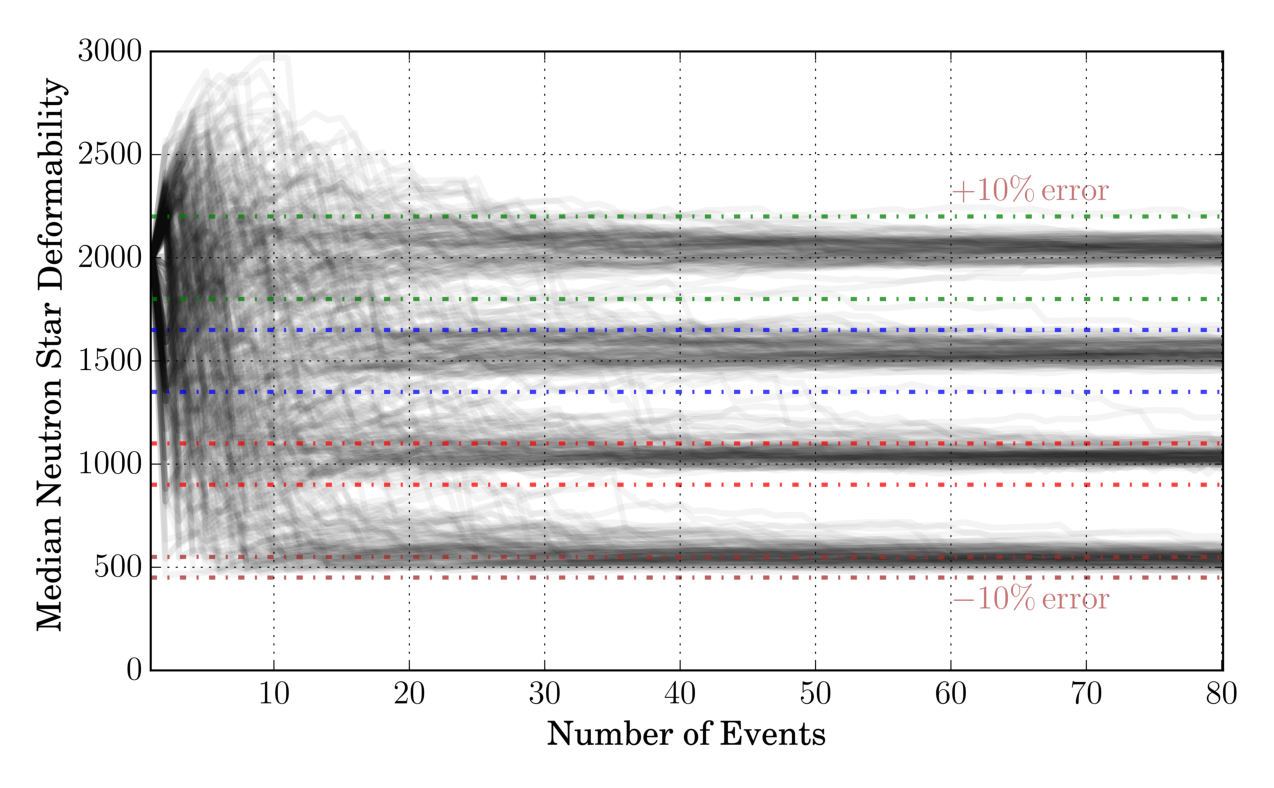
\includegraphics[trim=20 0 0 0, width=1.02\columnwidth]{plots/LambdaMedian_vs_N_AstroPopulation}
\caption{%
{\it Left:} This figure shows the median value of the recovered
probability distribution for $\lambdans$, as a function of the number of events
in the population $N$. There are four family of curves, one corresponding each
to $\lambdans=\{500,1000,1500,2000\}$, with $100$ independent populations
within each family. One curve in each family is highlighted in color, 
representing that it is the same population as was illustrated in
Fig.~\ref{fig:TT_Lambda_vs_N_L800_CI90_0}-\ref{fig:TT_Lambda_vs_N_CI90_0}.
In the same color we show $\pm 10\%$ error-bounds on $\lambdans$ with
horizontal dash-dotted lines. We observe that within $10-25$ observations, 
the median of the measured cumulative probability distribution for $\lambdans$
will lie within $10\%$ of the true value.
{\it Right:} This figure is identical to the left panel, with the only
difference that the BH masses in each population are restricted to lie
{\it outside} the astrophysical mass-gap (i.e. paradigm B). The difference that
we observe under this paradigm is that we need more ($30+$) events to achieve 
the same ($10\%$) measurement accuracy for populations with $\lambdans<1000$.
For more deformable neutron stars, $10-25$ events would suffice.
}
\label{fig:TT_LambdaMedian_vs_N_AllInOne}
\end{figure*}
%
% 
% \begin{figure*}
% \centering    
% \includegraphics[width=1.03\columnwidth]{plots/RelErrorLambdaMedian_vs_N.pdf}
% \includegraphics[width=1.03\columnwidth]{plots/LambdaCIWidths_vs_N.pdf}
% \caption{{\it Left}: In the main panel is shown the width of the measured $90\%$ 
% confidence interval for $\lambdans$, normalized by its true value,
%  as a function of the number of events observed $N$. In the inset, we
%  show the same measurement uncertainty, but not normalized, and on a 
%  logarithmic axis for $N$ as well.
% % 
%  From both the inset and the main plot, we find that for the first $3-4$ events
%  our measurement is prior limited. As $N$ increases, the uncertainty falls 
%  roughly as $1/\sqrt{N}$ with intermittent loud signals causing more rapid 
%  (than $1/\sqrt{N}$) narrowing of the confidence interval.
% %  
%  {\it Right}: This figure shows the fractional difference between the median
%  recovered value from the posterior probability distribution for $\lambdans$
%  as a function of $N$. Different curves correspond to different injected values
%  of $\lambdans$, and are shaded from light to dark in direct proportion. 
%  The horizontal dashed brown line marks $10\%$ deviation of the median from the 
%  true value.
% %  
% We find that within $\approx 10$ detections, the median measured value for
% $\lambdans$ would estimate the true value for the star with the remarkable 
% accuracy of $10\%$.
% }
% \label{fig:TT_LambdaError_vs_N_L500_2000_CI90_0}
% \end{figure*}
%LambdaCIWidths_vs_N_AllPopulations_Log_L
% 
%
% 
\begin{figure*}
\centering    
\includegraphics[width=0.8\columnwidth]{plots/LambdaCIWidths_vs_N_AllPopulations_Log_L2000.pdf}
\includegraphics[width=0.8\columnwidth]{plots/LambdaCIWidths_vs_N_AstroPopulations_Log_L2000.pdf}\\
\includegraphics[width=0.8\columnwidth]{plots/LambdaCIWidths_vs_N_AllPopulations_Log_L1500.pdf}
\includegraphics[width=0.8\columnwidth]{plots/LambdaCIWidths_vs_N_AstroPopulations_Log_L1500.pdf}\\
\includegraphics[width=0.8\columnwidth]{plots/LambdaCIWidths_vs_N_AllPopulations_Log_L1000.pdf}
\includegraphics[width=0.8\columnwidth]{plots/LambdaCIWidths_vs_N_AstroPopulations_Log_L1000.pdf}\\
\includegraphics[width=0.8\columnwidth]{plots/LambdaCIWidths_vs_N_AllPopulations_Log_L800.pdf}
\includegraphics[width=0.8\columnwidth]{plots/LambdaCIWidths_vs_N_AstroPopulations_Log_L800.pdf}\\
\includegraphics[width=0.8\columnwidth]{plots/LambdaCIWidths_vs_N_AllPopulations_Log_L500.pdf}
\includegraphics[width=0.8\columnwidth]{plots/LambdaCIWidths_vs_N_AstroPopulations_Log_L500.pdf}
\caption{%
These figures show the width of the $90\%$ confidence interval for $\lambdans$
(normalized by its true value), as a function of the number of observed events
$N$. The left column panels show populations sampled under paradigm A, which
allows BH masses to fall within the astrophysical mass-gap, while those on the
right show populations drawn under paradigm B which respects the mass-gap.
Each panel corresponds to a unique value of populations' $\lambdans$,
decreasing from $2000\rightarrow 500$ as we go from top to bottom. In each panel,
$100$ curves are shown, each corresponding to an independent population draw. The
one colored curve in each panel highlights the population used in
Fig.~\ref{fig:TT_Lambda_vs_N_L800_CI90_0}-\ref{fig:TT_Lambda_vs_N_CI90_0}.
The insets in each panel show the same information, with the ordinate {\it not}
normalized by the true value of $\lambdans$.
% 
We find that with approximately $25$ or so events, we begin to put
statistically meaningful constraints on $\lambdans$, restricting it to within
$\pm 50\%$ of the true value. We can expect to achieve this with a few years
of design aLIGO operation~\cite{Abadie:2010cfa}. Further tightening of the
confidence intervals will require $40+$ events.
}
\label{fig:TT_LambdaError_vs_N_L500_2000_CI90_0_AllInOne}
\end{figure*}
% 
% % 
% \begin{figure*}
% \centering    
% \includegraphics[width=.9\columnwidth]{plots/LambdaCIWidths_vs_N_AllPopulations_Log_L2000.pdf}
% \includegraphics[width=.9\columnwidth]{plots/LambdaCIWidths_vs_N_AllPopulations_Log_L1500.pdf}\\
% \includegraphics[width=.67\columnwidth]{plots/LambdaCIWidths_vs_N_AllPopulations_Log_L1000.pdf}
% \includegraphics[width=.67\columnwidth]{plots/LambdaCIWidths_vs_N_AllPopulations_Log_L800.pdf}
% \includegraphics[width=.67\columnwidth]{plots/LambdaCIWidths_vs_N_AllPopulations_Log_L500.pdf}
% \caption{ In the main panel is shown the width of the measured $90\%$ 
% confidence interval for $\lambdans$, normalized by its true value,
%  as a function of the number of events observed $N$. In the inset, we
%  show the same measurement uncertainty, but not normalized, and on a 
%  logarithmic axis for $N$ as well.
% % 
%  From both the inset and the main plot, we find that for the first $3-4$ events
%  our measurement is prior limited. As $N$ increases, the uncertainty falls 
%  roughly as $1/\sqrt{N}$ with intermittent loud signals causing more rapid 
%  (than $1/\sqrt{N}$) narrowing of the confidence interval.
% }
% \label{fig:TT_LambdaError_vs_N_L500_2000_CI90_0}
% \end{figure*}
% % 
% 




\textbf{Multiple identical sources at low SNR: }\label{s2:identical_multiple}
% 
We start with a crude calculation which tells us that approximately $8$ (or $16$) 
observations
of NSBH signals with $\rho\geq 10$ distributed uniformly in effective volume, would
give us similarly accurate a measurement of $\lambdans$ as would a single detection
with $\rho=50$ (or $\rho=70$). 


The approximation of using (only) the dominant $l=|m|=2$ multipoles of
gravitational-wave strain to construct the signal, ignoring other $l\neq 2$
multipoles, has the advantage of making various angle parameters 
associated with the source degenerate with its distance. As a result, source
distance, source sky location angles, and the inclination angle of
the binary's orbital angular momentum with respect to the detector,
all combine into a single ``effective distance'' $\deff$ that scales
out as the constant amplitude factor $1/\deff$ (constant because none
of the above parameters vary temporally for aligned-spin binaries).
% 
In order to consider multiple events, lets imagine a population uniformly
distributed in effective volume, i.e. within a sphere of radius 
$\deff^\mathrm{max}$. The radius of this sphere is set by the lowest SNR that 
is distinguishable from noise by LIGO searches. Now, divide the sphere into
$I$ shells of equal thickness. The radius of the $i$-th sphere would then
be $D_i = \deff^\mathrm{max} (i - 1/2)/I$. The measurement uncertainty in
$\lambdans$ scales inversely with SNR, and hence directly with the 
effective distance to the source. Therefore, if we have a measurement error 
$\sigma_0$ for a source located at $\deff = D_0$, the same error for the same
source located within the $i$-th shell would be 
$\sigma_i = \sigma_0 \dfrac{D_i}{D_0}$. The combined error from independent
measurements of $\lambdans$ for identical sources at different distances is
given by
\begin{equation}\label{eq:1oversigma}
\frac{1}{\sigma^2} = \sum_{i=1}^I \frac{N_i}{\sigma_i^2} = \left(\frac{D_0}{\sigma_0}\right)^2 \sum_{i=1}^I\frac{N_i}{D_i^2},
\end{equation}
where $N_i$ is the number of sources detected in the $i$-th shell.
% , and is a random
% variable, with its probability proportional to the volume of the shell, i.e.
% $$
% p(N_i) \propto \frac{V_i}{V_\mathrm{total}} \propto \dfrac{\left(\deff^\mathrm{max} \frac{i}{I}\right)^3 - \left(\deff^\mathrm{max} \frac{i-1}{I}\right)^3}{(\deff^\mathrm{max})^3} \propto \frac{1}{I^3} [i^3 - (i-1)^3].
% $$
% Therefore, the expected number of detections in the $i$-th shell would be
% $$
% \langle N_i\rangle = \frac{N}{I^3} [i^3 - (i-1)^3],
% $$
% where $N=\sum_{i=1}^I N_i$ is the total number of NSBH detections. $N$ is expected
% to be Poisson distributed around the mean detection rate
% $\mathcal{R}\equiv\langle N\rangle$, where $\mathcal{R}$ can vary from $0.6-1000$ per
% $\mathrm{Gpc}^3$ per year~\cite{Abadie:2010cfa}. If there are $n$ resulting detections
% a year per unit effective volume, then
% \begin{equation}
% \langle N\rangle = \int_0^{\deff^\mathrm{max}} 4\pi n D^2 \D D = \frac{4\pi}{3} n (\deff^\mathrm{max})^3,
% \end{equation}
% and
% \begin{eqnarray}
%  \langle \frac{1}{\sigma^2}\rangle &=& \left(\frac{D_0}{\sigma_0}\right)^2 \int_0^{\deff^\mathrm{max}} \frac{4\pi n D^2 }{D^2}\D D\\
%  &=& \left(\frac{D_0}{\sigma_0}\right)^2 4\pi n \deff^\mathrm{max},
% \end{eqnarray}
% where in the previous equation we have converted the summation in Eq.~\ref{eq:1oversigma} 
% to an integral. 
Continuing on this line of inquiry, Ref.~\cite{Markakis:2010mp} found the 
root-mean-square averaged measurement error from 
$\langle N\rangle:=\langle\sum N_i\rangle$ sources distributed uniformly in
effective volume within a sphere of radius $\deff^\mathrm{max}$ to be
\begin{equation}\label{eq:rmsSigmaIdenticalSources}
 \sigma_{avg} := \frac{1}{\sqrt{\langle1/\sigma^{2}\rangle}} = \frac{\sigma_0}{D_0} \deff^\mathrm{max} \frac{1}{\sqrt{3\langle N\rangle}},
\end{equation}
given a fiducial pair $(\sigma_0, D_0)$. It is straightforward to deduce from
Eq.~\ref{eq:rmsSigmaIdenticalSources}
that the same measurement certainty as afforded by a single
observation with a high SNR $\rho_c$ can be obtained from $N = \rho_c^2/300$ observations
uniformly distributed in effective volume with SNRs $\geq 10$. E.g., to get to the level 
of certainty afforded at SNR$=70$, we would need $49/3\approx 16-17$ realistic detections.

There are two main caveats to this rudimentary calculation, first outlined in 
Ref.~\cite{Markakis:2010mp}: (i) it applies to identical sources,
which is astrophysically next to impossible to achieve exactly, but could perhaps happen 
approximately; (ii) the combined average measurement error $\sigma_{avg}$ has been defined
as in the first equality in Eq.~\ref{eq:rmsSigmaIdenticalSources}. To overcome both,
we next perform a Bayesian population analysis.


\textbf{Astrophysical source population: }\label{s2:astro_multiple}
% 
Imagine that we have $N$ stretches of data, $d_1, d_2, \cdots, d_N$, each 
containing a single signal emitted by an NSBH binary. Each of these signals can
be characterized by the following binary parameters:
$\,\vec{\theta} = \{\mbh, \mns, \chibh, \chins, \rho\}\cup\{\lambdans\}$. Note
that we have folded in the luminosity distance, inclination angle of the 
binary's orbital angular momentum with respect to the plane of the detector,
and source's sky location angles into a single parameter $\rho$, which is the 
SNR of the received signal. This is possible because of our simplification of 
using only the dominant $l=|m|=2$ modes of the GW strain~\footnote{The 
$l=|m|=2$ multipoles of the GW strain, when decomposed in a spin $-2$ weighted
spherical harmonic basis, contain more than $99\%$ of the total signal power}
that makes various angle parameters completely degenerate with distance. 
Further, let $K$ denote all of our collective prior knowledge, except for 
expectations on binary parameters themselves, which enter the following 
calculation explicitly. For instance, $K$ includes our assumption that all
NS's in a single population have the same deformability parameter $\lambdans$, 
and its cumulative measurement is therefore possible.
% 
Using Bayes' theorem, the measured probability distribution function for 
$\lambdans$ from $N$ observations is given by~\footnote{%
Eq.~\ref{eq:lambdaMultiple} includes the following implicit factor to normalize
its right-hand side: $\dfrac{\prod_i p(d_i|K)}{\int p(\lambdans)\,p(d_1, d_2, \cdots, d_N | \lambdans; K)\,\D\lambdans}$}
\begin{equation}\label{eq:lambdaMultiple}
 p(\lambdans | d_1, d_2, \cdots, d_N; K) = p(\lambdans | K)^{1-N}\prod_{i=1}^N p(\lambdans | d_i, K),
\end{equation}
where $p(\lambdans|K)$ is the prior expectation for $\lambdans$, and all $N$ 
observations are taken to be mutually independent. A priori, we assume
that no particular value of $\lambdans$ is preferred over another, and 
$\lambdans\leq 4000$, i.e.
\begin{equation}\label{eq:lprior}
 p(\lambdans | K) = \dfrac{1}{4000}\,\mathrm{Rect}\left(\frac{\lambdans-2000}{4000}\right).
\end{equation}
% 
In the second set of terms in Eq.~\ref{eq:lambdaMultiple} (of the form 
$p(\lambdans | d_i, K)$), each is the probability distribution for $\lambdans$
inferred {\it a posteriori} from the \textit{i}-th observation in isolation. 
They are calculated by integrating
\begin{equation}\label{eq:margpost}
 p(\lambdans | d_i, K) = \int \D \vec{\theta}\, p(\vec{\theta}, \lambdans | d_i, K),
\end{equation}
where $p(\vec{\theta}, \lambdans | d_n, K)$ is the inferred joint probability 
distribution of all source parameters $\vec{\theta}\cup\{\lambdans\}$ for the 
$i$-th event, as given by Eq.~\ref{eq:postprob}. By substituting
Eq.~\ref{eq:lprior}-\ref{eq:margpost} into Eq.~\ref{eq:lambdaMultiple}, we
calculate the probability distribution for $\lambdans$ as measured using $N$
independent events.




Our goal is to understand the improvement in our measurement of $\lambdans$
with the number of recorded events. To do so, we simulate populations of $N$
observations each, and quantify what we learn from each successive observation 
using Eq.~\ref{eq:lambdaMultiple}. For each population, we determine how
rapidly our median estimate for $\lambdans$ converges to the true value,
and how rapidly our confidence intervals for the same shrink, with increasing
$N$. In order to generate each population, we first fix
the NS properties: (i) NS mass $\mns=1.35M_\odot$, (ii) NS spin $\chins=0$
and (iii) NS tidal deformability $\lambdans=$ fixed value chosen from
$\{500,800,1000,1500,2000\}$. Each event is generated independently, sampling
the remaining source parameters uniformly from the following ranges: (i)
mass-ratio $q\in[2,5]$, (ii) BH spin $\chibh\in[0, 0.75]$, (iii) effective 
distance from within a spherical volume whose radius is given by the lowest 
detectable SNR (which we take as $\rho=10$). We remind ourselves that
once binary parameters are fixed, there is a one-to-one mapping between
effective distance and SNR. Additionally, we consider an alternate population
paradigm (paradigm B, with paradigm A being the standard one described 
above), where populations are generated as above but further restricting
mass-ratios such that source BH masses lie {\it outside} the astrophysical 
mass-gap~\cite{Bailyn:1997xt,Kalogera:1996ci,Kreidberg:2012,Littenberg:2015tpa}.
Finally, in order to mitigate computational cost, we make an additional 
simplification. We perform full Bayesian parameter estimation for a set of 
simulated signals whose parameters are the vertices of the following regular
hypercubic grid (henceforth ``G''):
$q=\{2,3,4,5\}\times\chibh=\{-0.5,0,0.5,0.75\}\times\lambdans=\{500,800,1000,1500,2000\}\times\rho=\{10,20,30,50,70\}$.
The final population is given by substituting all of the $N$ events, generated
as above, with their respective nearest neighbours on the parameter grid G.


In Fig.~\ref{fig:TT_Lambda_vs_N_L800_CI90_0} we show illustrative results
for a single 
population of $N=80$ events. The neutron star deformability is fixed at
$\lambdans=800$ for all events. In the left panel, each curve shows the 
probability distributions for $\lambdans$ as inferred from $N$ events, with $N$
ranging from $1-80$. We also mark the $90\%$ confidence intervals associated
with each of the probability distribution curves. From the figure, we
can visualize information accumulation. The first few observations do not have
enough information to bound $\lambdans$ (with $90\%$ confidence) much more than
our prior from Eq.~\ref{eq:lprior} does. However, the median of these
cumulative distributions appears to track the true value of $\lambdans$ 
rapidly.
% 
In the right panel, we present information derived from the left panel.
The line-circle curve shows the measured median from $N$ observations, with
the latter on the $x$-axis. The pair of dashed (dotted) horizontal lines mark
$\pm25\%$ ($\pm50\%$) error bars. At each $N$, the range spanned by the 
filled region is the $90\%$ confidence interval deduced from the same 
events. This figure somewhat quantifies the qualitative deductions we made
from the left panel. We find that the measured median does track the true value
quickly, reaching $10\%$ accuracy with $10-15$ observations. With the same
information, our confidence intervals also shrink to $\pm 25\%$.
% 
In Fig.~\ref{fig:TT_Lambda_vs_N_CI90_0} we show further results from $4$
independent populations, with the source $\lambdans$ alone changing between
them. The sampled values, i.e.$\lambdans=\{500,1000,1500,2000\}$, 
range from the least to the most deformable neutron stars. As in the 
right panel of Fig.~\ref{fig:TT_Lambda_vs_N_L800_CI90_0}, the line-circle curves
track the median measured $\lambdans$, while the filled regions show
the associated $90\%$ confidence intervals. From the figure, we observe
the following: (i) the shrinkage of confidence interval widths with increasing
$N$ happens in a similar manner for all 
populations, (ii) within $5-10$ observations, median measured $\lambdans$ for
all populations lie within $\pm10\%$ of the true values, and (iii) it takes
approximately $20$ events to distinguish definitively (with $90\%$ confidence)
between deformable NSs with $\lambdans=2000$ and compact NSs with 
$\lambdans=500$, or equivalently to distinguish between hard, moderate and soft
nuclear equations of state. This is comparable to what has been found for
monolithic binaries of neutron stars~\cite{DelPozzo:13,Chatziioannou:2015uea,
Agathos:2015a}.



So far we have discussed individual realizations of NSBH populations. The 
underlying stochasticity of the population generation process makes it
difficult to draw generalized inferences (from a single realization) about the
measurability of $\lambdans$. We mitigate this by drawing multiple
realizations of population generation (i.e. multiple identically constructed
populations). Fig.~\ref{fig:TT_LambdaMedian_vs_N_AllInOne} shows the first
results for multiple populations. Lets focus on the left panel first. We
show the median measured value of $\lambdans$ from $100$ independent 
populations with fixed $\lambdans=2000$ as the top set of curves. The one 
highlighted (in green) curve corresponds to the population discussed above.
Similarly, we generate sets of $100$ populations with $\lambdans=500-1500$, and
show the median measured $\lambdans$ as four distinct groups of curves in
Fig.~\ref{fig:TT_LambdaMedian_vs_N_AllInOne} (with the single highlighted
curve in each group corresponding to
Fig.~\ref{fig:TT_Lambda_vs_N_L800_CI90_0}-\ref{fig:TT_Lambda_vs_N_CI90_0}).
Dash-dotted horizontal lines demarcate $\pm50\%$ error intervals around
the true $\lambdans$ values. All of these populations are drawn under
paradigm A (i.e. with BH masses allowed to sample the mass-gap that spans
$2-5M_\odot$).
% 
From the figure, we can conclude with a high likelihood that our measured
$\lambdans$ values will be within $10\%$ of the real value in $15-20$ events
for less deformable neutron stars with $\lambdans\leq 1000$, and in as few as
$10$ events for more deformable stars with $\lambdans\geq 1500$.
% 
The right panel of the figure is identical to the left panel, but drawn under
population paradigm B (no BHs alloewd within the mass-gap). Under this
paradigm, we expectedly find that information accumulation is slower. It would
take $20-40$ detections with $\rho\geq10$ under this paradigm, for our (median)
measured $\lambdans$ to lie within $10\%$ of the true value (fewer for 
more deformable NSs, as one would expect).
% 
This is a promising deduction, as one might expect to see $\mathcal{O}(10)$
events over a few years' timescale with design aLIGO~\cite{Abadie:2010cfa}.



Further, we investigate the statistical uncertainties associated with
$\lambdans$ measurements. We use $90\%$ confidence intervals as our measure of
the same. The left column of 
Fig.~\ref{fig:TT_LambdaError_vs_N_L500_2000_CI90_0_AllInOne} shows results
under paradigm A, where BH mass priors include the mass-gap. In each panel
we show the width of the $90\%$ confidence interval measured from $N$ events
(with $N$ on the $x$-axis), normalized by the true value of $\lambdans$ for
the population. In grey are shown results from each of $100$ population
realizations, with the single population highlighted in color corresponding
to the one we focused on in 
Fig.~\ref{fig:TT_Lambda_vs_N_L800_CI90_0}-\ref{fig:TT_Lambda_vs_N_CI90_0}.
The inset shows the same, except that the ordinate is {\it not} normalized by
the true value of $\lambdans$. From top to bottom, the population $\lambdans$
decreases from $\lambdans=2000\rightarrow 500$, corresponding to decreasingly
deformable NSs with softer equations of state. We observe the following:
(i) for moderately-hard to hard equations of state with $\lambdans\geq 1000$,
we can constrain $\lambdans$ within $\pm 50\%$ using only $10-20$ events, and
within $\pm 25\%$ with $25-40$ events; (ii) for softer equations of state with
$\lambdans<1000$, we will achieve the same accuracy with $20-30$ and $50+$ 
events, respectively; and (iii) for the first $5$ or so observations, our
measurement confidence spans the entire prior allowed range 
$\lambdans\in[0,4000]$, as shown by the plateauing towards the left edge in
each panel's inset.
% 
In the right column, each panel panel is identical to its corresponding left
one, with the difference that populations are drawn under paradigm B, which
does {\it not} allow for BH masses to fall within the mass-gap. We find that
for NSs with $\lambdans\leq 1000$, it would take $25-40$ events to
constrain $\lambdans$ within $\pm 50\%$ and $50+$ events to constrain it
within $\pm 25\%$. This is somewhat slower than paradigm A, as is to be
expected since here we preclude the lowest mass-ratios, which correspond to
signals with largest tidal signatures. For $\lambdans>1000$ we find that we
can constrain $\lambdans$ within $\pm 50\%$ with a similar number of events as
for paradigm A, but will need more ($30-40$, as compared to $25-40$) events
to further constrain it to within $\pm 25\%$ of the true value.
% 
These are some of the primary findings of this paper.


% Finally, we quantitatively explore the dependence of our statistical
% uncertainties for $\lambdans$ on the number of events, as well as on the true
% NS deformability itself. First, we will focus on the dependence on $N$. We
% assume a power-law dependence of the form
% $\delta\lambdans\propto\ 1/N^\alpha$. For each of the $100$ populations 
% for each of $\lambdans=500-2000$, we compute the exponent $\alpha$ as a
% function of the number of observed events $N$, and show it in 
% Fig.~\ref{fig:TT_PowerLawLambdaErrorVsN}. There are $100\times5=500$ curves
% on the figure, with one highlighted for each value of population's $\lambdans$.
% These highlighted values are only special in the sense that they correspond to
% populations discussed earlier in this section (c.f.
% Fig.~\ref{fig:TT_Lambda_vs_N_L800_CI90_0}-\ref{fig:TT_Lambda_vs_N_CI90_0}).
% We immediately observe two things, (i) there is a globally similar dependence
% on $N$ for all populations, and (ii) information accumulates {\it faster} than
% $1/\sqrt{N}$. In fact, we find that if
% $\delta\lambdans\propto\frac{1}{N^\alpha}$, $\alpha$ lines in the range
% $0.7_{-0.2}^{+0.2}$.
% % 
% Next, we focus on the dependence of $\delta\lambdans$ on $\lambdans$ of the
% population itself. As suggested by Fisher-matrix studies~\cite{Lackey:2013axa},
% and as for $N$, we assume the form $\delta\lambdans\propto\lambdans^\beta$.
% From each set of $100$ populations with a given $\lambdans$ value, we draw one
% at random, and form a set of $5$ similarly drawn populations, one for each of
% $\lambdans=\{500,800,1000,1500,2000\}$. With each set, we determine $\beta$
% for different number of observed events $N$. In all, we make $100$ independent
% $5-$population sets and show the value of $\beta$ measured from each in 
% Fig.~\ref{fig:TT_PowerLawLambdaErrorVsLambda}. We find that the assumed
% relation $\delta\lambdans\propto\lambdans^\beta$ gets fairly robust for 
% larger values of $N$, with $\beta$ converging to $\beta=0.5^{+0.33}_{-0.33}$.
% The fact that $0<\beta<1$ implies that the relative error
% $\delta\lambdans/\lambdans$ {\it decreases} with increasing $\lambdans$, while
% the absolute error {\it increases}.
% % 
% From these results, we conclude that the measurement uncertainty for
% $\lambdans$ after $N$ observations is
% \begin{equation}
%  \delta\lambdans\propto \dfrac{\lambdans^{0.5^{+0.33}_{-0.33}}}{N^{0.7_{-0.2}^{+0.2}}}.
% \end{equation}
% We also find that while these results are inferred from paradigm A populations,
% paradigm B gives very similar results.



To summarize, in this section we study the improvement in our measurement of 
NS deformability parameter $\lambdans$ with an increasing number of events. We
do so by simulating plausible populations of disrupting NSBH binaries (with
$\rho\geq 10$). We find that:
(i) for more deformable neutron stars (harder equation of states), the median
measured value of $\lambdans$ comes within $10\%$ of the true value with as 
few as $10$ events, while achieving the same accuracy for softer equations of 
state will take $15-20$ source detections; (ii) the statistical uncertainty
associated with $\lambdans$ measurement shrinks to within $\pm50\%$ with
$10-20$ events, and to within $\pm 25\%$ with $50+$ events, when source 
$\lambdans\geq 1000$; (iii) for softer equations of state, the same could take
$25-40$ and $50+$ events, respectively for the two uncertainty thresholds;
and (iv) if BHs really do observe the astrophysical mass-gap, the information
accumulation is somewhat slower than if they do not. We conclude that within
$20-30$ observations, aLIGO would begin to place very interesting bounds on 
the NS deformability, which would allow us to rule out or rank different
equations of state for neutron star matter.




%%%%%%%%%%%%%%%%%%%%%%%%%%%%%%%%%%%%%%%%%%%%%%%%%%%%%%%%%%%%%%%%%%%%%%%%%%%%%%%
\section{Discussion}\label{s1:discussion}
%%%%%%%%%%%%%%%%%%%%%%%%%%%%%%%%%%%%%%%%%%%%%%%%%%%%%%%%%%%%%%%%%%%%%%%%%%%%%%%


The pioneering terrestrial observation of gravitational waves by Advanced LIGO
harbingers the dawn of an era of gravitational-wave astronomy where 
observations, more than theory, would play the driving role. Binaries of 
compact stellar objects evolve under the radiation reaction force of emitting
gravitational waves.


Conventional astronomical methods have, to date, made observations of ~2500
NSs with masses between $1.25-2.1 M_\odot$~\cite{Lyne:2004cj,
Demorest:2010bx,2013Sci...340..448A,atnfcatalog,mcgillmagnetarcatalog,
stellarcollapsemass}, although
tightly clustered within $1.35\pm0.5M_\odot$~\cite{stellarcollapsemass}.
%
Observations of over 2500 NSs have shown that the spin of NSs
$|\vec{\chi}_\mathrm{NS}|$ have magnitudes that are $<1\%$~\cite{Miller:2014aaa}.
%
On the other hand, indirect observations of stellar-mass BHs place their
masses between $5-35M_\odot$, with their spin angular momenta 
$|\vec{\chi}_\mathrm{BH}|$ ranging from small to nearly extremal (Kerr) values
(see, e.g., Refs.~\cite{McClintockEtAl:2006,Miller:2009cw,Gou:2014una} for 
examples of nearly extremal estimates of BH spins, Refs.~\cite{McClintock:2013vwa,
Reynolds:2013qqa} for recent reviews of astrophysical BH spin measurements,
and Figure 5 of Ref.~\cite{Miller:2014aaa} for a comparison of NS and BH spins).

\prayush{[PK: To be continued after revision of the introduction.]}

\prayush{
We find that non-inclusion of tidal effects leads to systematic biases in
the measurement of non-tidal parameters. Consider first the binary chirp 
mass $\mchirp:=M\eta^{3/5}$ where $M$ is the binary total mass, and 
$\eta:=\mbh\mns/M^2$ is the dimensionless mass-ratio. We find that for
realistic (moderate) SNRs, i.e. $\rho\lesssim 30$, not including tidal
effects introduces a barely measurable bias that remains below $50\%$
of the statistical uncertainty of the $\mchirp$ measurement itself.
For higher signal strengths, we find that the underlying statistical
uncertainty decreases enough for the systematic bias to become comparable
to it for $\rho=50-70$ and higher. This is expected because chirp mass is fairly
accurately determined by the inspiral, where tidal effects are weak.
Next, we consider the mass-ratio $\eta$. We find that only if the NS is quite
deformable (with $\lambdans=2000$), {\it and} has a companion BH whose mass
is $\mbh\lesssim 4.5M_\odot$ (i.e. in the astrophysical ``mass-gap''~\cite{
Bailyn:1997xt,Kalogera:1996ci,Kreidberg:2012,Littenberg:2015tpa}),
will the systematic bias in $\eta$ measurement become comparable to its
statistical uncertainties at SNRs $\rho\leq 30$. For SNRs $\rho\gtrsim30$,
however, not including tidal effects is very likely to {\it significantly} bias
the mass-ratio estimate for NSBH binaries. Finally, we consider the spin on the
black hole $\chibh$. We find that $\chibh$ measurements are affected in a similar
way to $\eta$. By not including tidal effects, we compromise our measurement of
$\chibh$ significantly only if signal $\rho\gtrsim 30$. 
%
Overall, we learn an important thing. Bayesian parameter estimation algorithms
aimed at identifying NSBH binaries with low latency in order to alert 
electromagnetic (EM) observers in time to establish a possible coincident 
observation of a GRB~\cite{2012A&A...541A.155A,Singer:2014qca,Singer:2015ema,
Pankow:2015cra} can use BBH templates to look for NSBH systems with aLIGO.
This is so because the primary requirement of the EM follow-up effort is rapid
classification of a binary as an NSBH system, which can be achieved just as 
easily with BBH templates, purely on the basis of the smaller component's mass.
Another conclusion we draw is that detection searches are unaffected by the
choice of ignoring tidal effects in matched-filtering templates.
}


\prayush{
The choices that determine the population are important here,
and were made as follows. Neutron star mass is fixed for signals at
$1.35M_\odot$, and its spin $\chins=0$. Black hole mass is sampled uniformly
from the range $[2,5]\times 1.35=[2.7, 6.75]M_\odot$. Our choice here is given
by the intersection set of the mass range that allows for neutron star disruption
and the range supported by the waveform model LEA+~\cite{Foucart2012,
Foucart:2013a,Lackey:2013axa}. Black hole spin is sampled uniformly from the
{\it aligned} range, i.e. $\chibh\in[0,+1]$. The true deformability is fixed
once per population, sampled uniformly from the range $\lambdans\in[0,2000]$.
In order to keep the computational cost tractable, we make a further 
approximation.
%
\textbf{%
We inject signals into zero noise at different SNRs and recover
their parameters from Bayesian inferencing for a fixed set of binaries,
whose parameters lie on a uniform grid given by:
$q=\{2,3,4,5\}\times\chibh=\{-0.5,0,0.5,0.75\}\times\lambdans=\{500,800,1000,1500,2000\}\times\rho=\{10,20,30,50,70\}$.
% 
Once the population parameters been selected, each event's parameters are
replaced by their nearest neighbor in the above set.
}
We make sure that this approximation is conservative by keeping our population
sampling ranges within the conservative side of the range spanned by the above
set. With the caveats laid out, we report our results in
Sec.~\ref{s1:multiple_observations}.
}


\prayush{
In addition, we probe two paradigms, one
that allows for BH masses to lie within the astrophysical mass-gap (paradigm
A), and one that does not (paradigm B).
% 
For paradigm A, we find the following: (i) for the softer equations of state
that result in less deformable neutron stars, $15-20$ detections are sufficient
for our median measured value of $\lambdans$ to lie within $10\%$ of the true
value. (ii) For NSBH populations with more deformable NSs
($\lambdans\geq 1000$), the same is achievable within as few as $10$ realistic
observations. (iii) The statistical uncertainty associated with $\lambdans$
measurement can be restricted to be within $\pm50\%$ using $10-20$ observations
when $\lambdans\geq 1000$), and using $25-40$ observations for softer equations
of state. All of the above is possible within a few years of design
aLIGO operation~\cite{Abadie:2010cfa}, if astrophysical BHs do indeed have
masses between $\leq 5M_\odot$ (i.e. in the mass-gap). However, further
restricting $\lambdans$ will require $50+$ NSBH observations.
% 
For paradigm B, we find the information accumulation to be somewhat slower.
While the quantitative inferences for $\lambdans\geq1000$ populations are
not affected significantly, we find $\mathcal{O}(10-20)\%$ more events are
required to attain the same measurement accuracy as under paradigm A.
% 
We conclude that within as few as $20-30$ observations of disruptive NSBH
mergers, aLIGO will begin to place interesting bounds on NS deformability.
This, amongst other things, will allow us to rank different equations of 
state for neutron star matter from most to least likely, with a few years'
time-scale.
}

\red{
MOVE towards end of SUMMARY, into ``Future work''.
}
\prayush{
Also note
that more a recent work that improves upon the waveform model we use in this
study has been published~\cite{Pannarale:2015jka}, but it provides only an 
amplitude model which needs to be (in future) augmented with a compatible
phase model. In addition, accuracy of the underlying numerical simulations 
used to calibrate the waveform model used here have not been verified against 
independent codes so far.
It is therefore difficult to assess the combined modeling error and its effect
on our results. they are, therefore, limited by the limitations of our
waveform model. However, we expect the combined effect of modeling errors to
not change our qualitative conclusions.
}


%%%%%%%%%%%%%%%%%%%%%%%%%%%%%%%%%%%%%%%%%%%%%%%%%%%%%%%%%%%%%%%%%%%%%%%%%%%%%%%
% Acknowledgments
%%%%%%%%%%%%%%%%%%%%%%%%%%%%%%%%%%%%%%%%%%%%%%%%%%%%%%%%%%%%%%%%%%%%%%%%%%%%%%%
\begin{acknowledgments}
We thank Ben Lackey, Francesco Pannarale, Francois Foucart, and Duncan Brown
    for helpful discussions. We gratefully acknowledge support
  for this research at CITA from NSERC of Canada, the Ontario Early 
  Researcher Awards Program, the Canada Research
  Chairs Program, and the Canadian Institute for Advanced Research; at
  Caltech from the Sherman Fairchild Foundation and NSF grants
  PHY-1404569 and AST-1333520; at Cornell from the
  Sherman Fairchild Foundation and NSF grants PHY-1306125 and
  AST-1333129; and at Princeton from NSF grant PHY-1305682 and the
  Simons Foundation.  Calculations were performed at the Vulcan
  supercomputer at the Albert Einstein Institute;
  H.P. and P.K. thank the Albert-Einstein Institute,
  Potsdam, for hospitality during part of the time where this research
  was completed.
\end{acknowledgments}

%%%%%%%%%%%%%%%%%%%%%%%%%%%%%%%%%%%%%%%%%%%%%%%%%%%%%%%%%%%%%%%%%%%%%%%%%%%%%%%
\begin{appendix}



\section{Phenomenology of $\lambdans$ measurement errors}
% 
\begin{figure}
\centering    
\includegraphics[width=1.05\columnwidth]{plots/PowerLawCoefficient_LambdaErrorvsN_vs_N.pdf}
\caption{%
Assuming a power-law dependence of the measurement error on the number of
events: $\delta\lambdans\propto 1/N^\alpha$, we show $\alpha$ in this figure
as a function of the number of observed events $N$. Shown are five families
of $100$ population draws each, with each family corresponding to one of
$\lambdans=\{500,800,1000,1500,2000\}$. Each grey curve corresponds to one
of these $100\times5 = 500$ populations. The thicker curves, one from each
family, shows the population we discussed in
Fig.~\ref{fig:TT_Lambda_vs_N_L800_CI90_0}-\ref{fig:TT_Lambda_vs_N_CI90_0}.
We find that a power-law is a good approximation for the concerned dependence,
and information accumulates {\it faster} than $1/\sqrt{N}$. We estimate
$\alpha\simeq 0.7^{+0.2}_{-0.2}$.
}
\label{fig:TT_PowerLawLambdaErrorVsN}
\end{figure}
%
% 
\begin{figure}
\centering    
% \includegraphics[width=1.03\columnwidth]{plots/LambdaRelErrorBars_vs_Lambda_AllPopulations_N80_Log.pdf}
\includegraphics[width=\columnwidth]{plots/PowerLawCoefficient_LambdaErrorvsLambda_vs_N_AllPopulations.pdf}
\caption{%
In this figure, which is similar to Fig.~\ref{fig:TT_PowerLawLambdaErrorVsN},
we quantify the dependence of $\delta\lambdans$ on $\lambdans$ itself. Of 
the five families of simulated NSBH populations, we construct $100$
independent sets taking one population from each family. With each of 
these $100$ sets, and assuming a power-law dependence:
$\delta\lambdans\propto\lambdans^\beta$, we estimate $\beta$ and show it in
this figure as a function of the number of observed events $N$.
% 
We find that $\beta$ can be estimated to lie within $[1/6,5/6]$ with a
likely value close to $1/2$. Since $0<\beta<1$, the relative error
$\delta\lambdans/\lambdans$ {\it decreases} as the star gets more 
deformable, while the absolute error $\delta\lambdans$ {\it increases}.
}
\label{fig:TT_PowerLawLambdaErrorVsLambda}
\end{figure}
% 
Finally, we quantitatively explore the dependence of our statistical
uncertainties for $\lambdans$ on the number of events, as well as on the true
NS deformability itself. First, we will focus on the dependence on $N$. We
assume a power-law dependence of the form
$\delta\lambdans\propto\ 1/N^\alpha$. For each of the $100$ populations 
for each of $\lambdans=500-2000$, we compute the exponent $\alpha$ as a
function of the number of observed events $N$, and show it in 
Fig.~\ref{fig:TT_PowerLawLambdaErrorVsN}. There are $100\times5=500$ curves
on the figure, with one highlighted for each value of population's $\lambdans$.
These highlighted values are only special in the sense that they correspond to
populations discussed earlier in this section (c.f.
Fig.~\ref{fig:TT_Lambda_vs_N_L800_CI90_0}-\ref{fig:TT_Lambda_vs_N_CI90_0}).
We immediately observe two things, (i) there is a globally similar dependence
on $N$ for all populations, and (ii) information accumulates {\it faster} than
$1/\sqrt{N}$. In fact, we find that if
$\delta\lambdans\propto\frac{1}{N^\alpha}$, $\alpha$ lines in the range
$0.7_{-0.2}^{+0.2}$.
% 
Next, we focus on the dependence of $\delta\lambdans$ on $\lambdans$ of the
population itself. As suggested by Fisher-matrix studies~\cite{Lackey:2013axa},
and as for $N$, we assume the form $\delta\lambdans\propto\lambdans^\beta$.
From each set of $100$ populations with a given $\lambdans$ value, we draw one
at random, and form a set of $5$ similarly drawn populations, one for each of
$\lambdans=\{500,800,1000,1500,2000\}$. With each set, we determine $\beta$
for different number of observed events $N$. In all, we make $100$ independent
$5-$population sets and show the value of $\beta$ measured from each in 
Fig.~\ref{fig:TT_PowerLawLambdaErrorVsLambda}. We find that the assumed
relation $\delta\lambdans\propto\lambdans^\beta$ gets fairly robust for 
larger values of $N$, with $\beta$ converging to $\beta=0.5^{+0.33}_{-0.33}$.
The fact that $0<\beta<1$ implies that the relative error
$\delta\lambdans/\lambdans$ {\it decreases} with increasing $\lambdans$, while
the absolute error {\it increases}.
% 
From these results, we conclude that the measurement uncertainty for
$\lambdans$ after $N$ observations is
\begin{equation}
 \delta\lambdans\propto \dfrac{\lambdans^{0.5^{+0.33}_{-0.33}}}{N^{0.7_{-0.2}^{+0.2}}}.
\end{equation}
We also find that while these results are inferred from paradigm A populations,
paradigm B gives very similar results.


\end{appendix}
%%%%%%%%%%%%%%%%%%%%%%%%%%%%%%%%%%%%%%%%%%%%%%%%%%%%%%%%%%%%%%%%%%%%%%%%%%%%%%%




%%%%%%%%%%%%%%%%%%%%%%%%%%%%%%%%%%%%%%%%%%%%%%%%%%%%%%%%%%%%%%%%%%%%%%%%%%%%%%%
\section*{References}
%%%%%%%%%%%%%%%%%%%%%%%%%%%%%%%%%%%%%%%%%%%%%%%%%%%%%%%%%%%%%%%%%%%%%%%%%%%%%%%
\bibliography{References/References}

\end{document}
